\documentclass[a4paper, 12pt, oneside, toc=listofnumbered, bibliography=totoc]{scrbook}
\usepackage[hyphens,spaces,obeyspaces]{url}
\usepackage[sorting = none, backend=bibtex]{biblatex}
\usepackage[german]{babel}
\usepackage[T1]{fontenc}
\usepackage[utf8]{inputenc}
\usepackage[hidelinks]{hyperref}
\usepackage{graphicx}
\usepackage{subcaption}
\usepackage{epstopdf}
\usepackage{lmodern}
\usepackage{float}
\usepackage{acronym}
\usepackage{booktabs}
\usepackage{caption}
\usepackage{csquotes}
\usepackage{enumitem}
\usepackage{fancyhdr}
\usepackage{url}
\usepackage{listings}
\usepackage[table]{xcolor}
\usepackage{wrapfig}
\usepackage{forest}
\usepackage{tabularx}
\usepackage{colortbl}
\usepackage{booktabs}
\usepackage[onehalfspacing]{setspace}
\usepackage{amsmath}
\usepackage{threeparttable}
\usepackage[german]{cleveref}
\usepackage{parskip}

\renewcommand*{\headfont}{\normalfont}
\renewcommand*{\multicitedelim}{\addsemicolon\space}
\renewcommand*{\headrulewidth}{0pt}
\renewcommand*{\arraystretch}{1.5}
\setlength{\parskip}{1.5ex}
\makeatletter
% define new boolean conditional switch for whether
% the abstract is being typeset
\newif\ifabstract
% redefine `\chapter` so it only starts a new page if not typesetting
% the abstract; sets abstract conditional to false after doing so
\renewcommand\chapter{\ifabstract\relax\else%
	\if@openright\cleardoublepage\else\clearpage\fi%
	\fi
	\abstractfalse%
	\thispagestyle{plain}%
	\global\@topnum\z@
	\@afterindentfalse
	\secdef\@chapter\@schapter}

% command for putting the title and name above the abstract; switches
% abstact boolean to true for next `\chapter*` command...
\newcommand{\conclusion}{
	\if@openright\cleardoublepage\else\clearpage\fi
		\begin{center}
			\textbf{\larger{Summary}}\par
			\emph{Hier kommt nach der Fertigstellung der Arbeit noch eine Zusammenfassung der Arbeit mit ein oder mehreren Sätzen hin. Hier kommt nach der Fertigstellung der Arbeit noch eine Zusammenfassung der Arbeit mit ein oder mehreren Sätzen hin. Hier kommt nach der Fertigstellung der Arbeit noch eine Zusammenfassung der Arbeit mit ein oder mehreren Sätzen hin2. }\par
		\end{center}

	\abstracttrue}
\makeatother
\lstset
{
         basicstyle=\footnotesize\ttfamily,
         numbers=left,               	% Ort der Zeilennummern
         numberstyle=\tiny,          	% Stil der Zeilennummern
%         stepnumber=2,               	% Abstand zwischen den Zeilennummern
         numbersep=5pt,              	% Abstand der Nummern zum Text
         tabsize=2,                  	% Groesse von Tabs
         extendedchars=true,
         breaklines=true,            	% Zeilen werden Umgebrochen
         keywordstyle=\color{red},
            frame=b,
 %        keywordstyle=[1]\textbf,    	% Stil der Keywords
 %        keywordstyle=[2]\textbf,
 %        keywordstyle=[3]\textbf,
 %        keywordstyle=[4]\textbf, \sqrt{\sqrt{}}
         stringstyle=\color{white}\ttfamily,
         showspaces=false,
         showtabs=false,
         xleftmargin=27pt,
         framexleftmargin=27pt,
         framexrightmargin=5pt,
         framexbottommargin=4pt,
%         backgroundcolor=\color{lightgray},
         showstringspaces=false      	% Leerzeichen in Strings anzeigen ?
}
\addbibresource{Bachelorarbeit.bib}
\setuptoc{toc}{numbered}

\begin{document}
	\frontmatter
	\def\doctype{Bachelorarbeit}
\def\title{Vorgehensweise zur Implementierung der VDMA Spezifikation „OPC UA for Machinery (OPC 40 001)“ in Maschinen und IT-Systemen erarbeiten}
\def\author{Rico Kursidem}
\def\supervisor{Dipl. Ing (FH) Michalowski}
\def\supervisortwo{Prof. Dr. Mielebacher}

\begin{titlepage}

\vspace{10mm}

\begin{center}
	
	\vspace{5mm}
	\huge \title
	
	\vspace{34pt}
	\large \doctype
		
	\vspace{30pt}	
	\small Angewandte Informatik \\
	\large Duale Hochschule Baden-Württemberg Mosbach \\
	\small Studienpartner \\
	\large AZO GmbH \& Co. KG \\
    \vspace{35pt}
    
    
\includegraphics[height=2.5cm]{prefix/image/logo-dhbw.eps}
    
\includegraphics[height=2.5cm]{prefix/image/logo-azo.png}
	
	\vspace{40pt}	
	\small von \\
	\large \author \\
	\small betreut von \\
	\large \supervisor \\
	\small und \\
	\large \supervisortwo

\end{center}

\vspace{75pt}


\vspace{49.7pt}

\fancypagestyle{empty}{
  \fancyhf{}
  \fancyfoot[C]{\today}
}

\end{titlepage}
	\chapter*{Abkürzungsverzeichnis} 
\begin{acronym}
	%A
	\acro{API}{Advanced Programming Interface}
	%B
	%C
	\acro{COM}{Component Object Model}
	%D
	\acro{DCOM}{Distrebuted Component Object Model}
	%E
	\acro{ERP}{Enterprse Recource Planning}
	%F
	%G
	%H
	\acro{HMI}{Human Maschine Interface}
	%I
	\acro{IoT}{Internet of Things}
	%J
	%K
	%L
	%M
	\acro{M2M}{Maschine-zu-Maschine}
	\acro{MES}{Manufacturing Execution System}
	\acro{MQTT}{Message Queuing Telemetry Transport}
	%N
	%O
	\acro{OPC UA}{Open Platform Communications Unified Architecture}
	%P
	%Q
	%R
	%S
	\acro{SOA}{Service orientierte Architektur}
	%T
	\acro{TCP/IP}{Transmission Control Protocol/Internet Protocol}
	%U
	\acro{UMATI}{Universal machien technology interface}
	%V
	\acro{VDMA}{Verband Deutscher Maschinen- und Anlagenbau}
	\acro{VDW}{Verein Deutscher Werkzeugmaschinenfabriken e.V. }
	%W
	%X
	%Y
	%Z
\end{acronym}
	\tableofcontents
	\listoffigures
	%\listoftables
	%\lstlistoflistings
	\nocite{*}

	
	
	\chapter*{Abstract}
	
	\section*{Deutsch}
	
	\section*{English}
	
	
	\mainmatter
	\pagebreak
%	\conclusionpng
	\chapter{Einführung}\label{ch:Einführung}
	% (4 Seiten)
	
	Die moderne Welt wird zunehmend vernetzter. Unternehmen weiten ihre Wertschöpfungsketten global aus und erzeugen so ein weltweites Abhängigkeitsnetz. Unternehmen erweitern Ihren Kundenmarkt auf die gesamte Welt und beziehen von überall Zulieferungen. In der Industrie ist es dabei besonders wichtig, dass alle Teilnehmer an Wertschöpfungsketten, Arbeitsgruppen und Verträgen dasselbe Verständnis von Daten haben. Um ein weltweit, einheitliches und unmissverständliches Kommunikationssystem zu ermöglichen, werden Standards verwendet. In Zeiten der Industrie 4.0 nehmen Standardisierungen einen noch wichtigeren Platz ein als zuvor. Da Anlagen immer mehr aus Maschinen verschiedenster Hersteller zusammengesetzt sind, ist ein gemeinsamer übergreifender Kommunikationsstandard besonders wichtig, um eine fehlerfreie, effiziente und wirtschaftliche Produktion zu ermöglichen.
	
	Standardisierung wird verwendet, um effizienteren Austausch und effektivere Prozesse durchzuführen. Ein sehr altes Beispiel sind Sprachen. Eine Menge an Regeln, welche zur Kommunikation genutzt werden, auf die sich alle Teilnehmenden geeinigt haben. In dieser Arbeit soll es um die Standardisierung im Bereich der \ac{M2M} Kommunikation gehen. Durch die Herausforderungen von Industrie 4.0 kann ein guter Standard die Integration mehrerer Systeme vereinfachen und Kosten sparen.
	
	In der M2M Kommunikation existieren bereits Standards, die schon vor Industrie 4.0 entworfen wurden. Dazu gehört \ac{OPC UA}. \ac{Umati} baut auf diesem Standard auf und definiert weitere Aspekte wie beispielsweise eine Plug \& Play Umgebung. Das Ziel von \ac{Umati} ist es, die zahlreichen Implementationen von OPC UA Schnittstellen zu standardisieren und zusammenzufassen, um so für Produzenten von Anlagen und Software einen gemeinsamen Standard zu finden. Das Ziel dieser Arbeit ist \ac{Umati} zu analysieren, die Implementation dieses Standards zu erforschen und ein Proof-of-Concept zu entwickeln, der die Fähigkeiten dieser Schnittstelle demonstriert.
	
	\section{Problemstellung und Ziel}
	
	% (1-2 Seiten)
	
	 Durch die zunehmende Automatisierung der Produktion und Fertigung stehen viele Produzenten vor der Aufgabe, zahlreiche Maschinen verschiedenster Hersteller in ihren Fertigungsprozess zu integrieren. Viele dieser Maschinen nutzen verschiedene Kommunikationsprotokolle, Datenformate und Schnittstellen, welche die Integration dieser diversen Systeme erschwert. Durch eine komplizierte Integration kann Vendor Lock-in entstehen. Dieses Konzept beschreibt die Bindung eines Kunden an einen Anbieter, da dieser eine Technologie oder Kommunikationsstrategie integriert, die andere Hersteller nicht oder nur extrem schwer integrieren können. Dies führt zu weniger Flexibilität und Kontrolle für den Kunden über das Projekt und steigert dessen Kosten. Um dieses Problem zu lösen, müssen sich die Produzenten zu einem Standard zusammenfinden und die Interoperabilität ihrer Systeme zu gewährleisten. \cite{mielebacher_verteilte_2021}
	 
	 Für AZO als Anlagenproduzent ist es von großem Interesse, mit Anlagen und Maschinen anderer Hersteller kommunizieren zu können und dabei die Integration einfach zu realisieren. Für Entwickler von \ac{MES} bedeutet die Standardisierung von Kommunikationsprotokollen eine schnellere und einfachere Entwicklung, was zu niedrigeren Entwicklungskosten führt und die Robustheit der Systeme erhöht. AZO nimmt an der Entwicklung von \ac{Umati} teil, um diese Standardisierung zu erreichen. Dieser Standard möchte die Schnittstellen für die Kommunikation zwischen Maschinen und mit der darüber liegenden Datenverarbeitung definieren und basiert auf dem offenen Standard \ac{OPC UA}.
	 
	 Das Ziel dieser Arbeit ist es, \ac{Umati} in einem Testumfeld anhand eines Proof-of-Conzept aufzubauen. Um dies zu erreichen, soll zunächst eine Marktanalyse durchgeführt werden, um mögliche Lösungen zum Versenden und Empfangen von Daten zwischen Maschine und \ac(MES) zu finden. Diese sollen anhand von selbst entwickelten Kriterien abgewogen und bewertet werden. Die vielversprechendsten Umsetzungen sollen in einem Testsystem implementiert werden und für zukünftige Demonstrationen auf Messen für AZO zur Verfügung gestellt werden.
	 
	 Dabei sollen zwei Systeme entstehen. Der VDMA bietet ein Web-Dashboard unter umati.app an, auf dem Zahlreiche Hersteller ihre Maschinen bereits Anbinden. Hier soll eine Simulierte Maschine von AZO ebenfalls dargestellt werden. Außerdem soll eine Interne Demonstration aufgebaut werden, die eine umatifähige Maschine in die bestehende Infrastruktur Integriert und die Informationen Visualisieren kann.
	
	\section{Unternehmen}
	
	 Diese Arbeit wird mit dem Dualen Partner \textit{AZO Gmbh \& Co. KG} durchgeführt. AZO bietet maßgeschneiderte Lösungen für die automatisierte Förderung, Lagerung und Dosierung von Rohstoffen weltweit an. Dabei werden Anlagen für die Bereiche der Chemie-, Nahrungsmittel-, Pharma-, Kosmetik und Kunststoffindustrie gefertigt. Diese Projekte umfassen die Planung, Fertigung und Montage sowie die Automatisierung der Anlagen.
	 
	 AZO entwickelt ein eigenes MES-System ACAS, welches die Kommunikation zwischen Anlagen von AZO, aber auch Anlagen von anderen Herstellern, mit den Kunden vereinheitlichen und verbessern soll. Dabei soll ein umfassendes System entstehen, welches Steuerung, Visualisierung und Überwachung der Produktion übernehmen und in einer zentralen Software bündeln soll.
	 
	 ACAS entsteht in der Entwicklungsabteilung, welche ebenfalls an dieser Arbeit beteiligt ist. Sie fokussiert sich auf die Automatisierung von AZO Anlagen im Bereich von SPS, Steuerungen bis zur Datenverarbeitung und Erhebung auf abstrahierter Ebene. 
	
	\section{Forschungsfragen}
	
	Die Standardisierung der Integration von verschiedensten Maschinen ist nötig und kann zu verstärkten Effizienzsteigerungen und Aufwandsersparnis führen. Für Anlagenbauer verspricht die Nutzung von \ac{Umati}, diese Integration in einen schnellen und effizienten Prozess zu wandeln. Um das Potenzial von \ac{Umati} zu evaluieren, wurden folgende Schwerpunkte betrachtet:
	
	\begin{itemize}
		\item \textbf{Q1}: Welche Herausforderungen ergeben sich bei der Umsetzung von \ac{Umati}?
		\item \textbf{Q2}: Welche Lösungen zur Umsetzung eines Prototypen von \ac{Umati} sind am Wirtschaftlichsten?
		\item \textbf{Q3}: Wie kann die Datenkommunikation zwischen Anlage und Visualisierungsplattform bestmöglich implementiert werden?
	\end{itemize}
	
	\section{Aufbau der Arbeit}
	
	Zu Beginn der Arbeit werden alle Grundlegenden Technologien und Themenbereiche beschrieben, die zum Verständnis benötigt werden (Kapitel \ref{ch:Grundlagen}). Daraufhin werden die Methodiken beschrieben, mit denen die Informationen für diese Arbeit erhoben wurden (Kapitel \ref{ch:Methodiken}). Im Hauptteil der Arbeit (Kapitel \ref{ch:Ergebnisse}) werden die Vorbereitenden Schritte für die Projekte sowie deren Durchführung behandelt. Die Implementation der Programme wird in Kapitel \ref{ch:Implementierung} in zwei Teilen behandelt, wobei die Implementation des Firmeninternen Prototyps aus Kapitel \ref{ch:Implementierung-Intern} auf die Ergebnisse aus Kapitel \ref{ch:Implementierung-Web} stützt. Die Arbeit schließt mit einer Diskussion der gefundenen Ergebnisse und einem Fazit (Kapitel \ref{ch:Diskussion_Fazit}).
	
	% TODO: Messematerial wenn in kapitel behandelt noch anhängen
	
\chapter{Grundlagen}\label{ch:Grundlagen}
	% (16 Seiten)
	
	% Stand der Technik
	
	
	\section{OPC UA}
	
	%Einführung
	\ac{OPC UA} ist ein unternehmensunabhängiger, offener Standard zur Kommunikation von Informationen und Daten zwischen Maschinen im industriellen Umfeld. Das Protokoll wurde 2008 von der OPC Foundation veröffentlicht und nimmt sich zur Aufgabe, die Interoperabilität von Systemen zu fördern. Es verwendet eine \ac{SOA} und kann auf verschiedensten Betriebssystemen verwendet werden. OPC UA ist sehr gut skalierbar und kann deshalb als Kommunikationsprotokoll bei kleinen \ac{IoT} Systemen als auch bei komplexen Cloud-Systemen zur Anwendung kommen. 
	 
	 %Server-Client Modell
	OPC UA baut auf einem Server-Client-Modell auf, wobei der Client die Anfragen an den Server senden muss. Der Client fragt den Server nach Daten und analysiert diese während der Server die Daten der dahinterliegenden Anlagen in übertragbare Strukturen bringt und sie zur Verfügung stellt. Da der jeder Client an mehreren Servern Daten erheben kann, wird das System gut skalier- und erweiterbar.
	
	%Interoperabilität
	Das Ziel von OPC UA und auch im weitergetragenen Sinne von \ac{Umati} ist das Erreichen von Interoperabilität von Maschinen im industriellen Bereich. Interoperabilität beschreibt die Standardisierung von Kommunikation zwischen Systemen. Allgemein kann diese in 4 Stufen eingeteilt werden, wobei jede Ebene auf die darunterliegende aufbaut. Im Schaubild \ref{fig:Interoperabilität} sind die vier Ebenen strukturelle, syntaktische, semantische und organisatorische Interoperabilität abgebildet.
	 
	 \begin{figure}[H]
	 	\centering
	 	\includegraphics[width=0.9\textwidth]{res/diagramms/Interoperabilität.pdf}
	 	\caption{Die vier Ebenen der Interoperabilität}
	 	\label{fig:Interoperabilität}
	 \end{figure}
	 
	 % Ebene 1
	 Die strukturelle Interoperabilität beschreibt Verbindungen zwischen den Systemen, weshalb sie auch oft als Konnektivität bezeichnet wird. Der Datenaustausch kann nur erfolgen, wenn die beteiligten Systeme miteinander verbunden sind und ein geeignete Schnittstelle implementieren. Diese Verbundenheit kann über ein Netzwerk mit TCP/IP oder HTTP erreicht werden oder kann ein Übertragungsmedium wie USB festlegen. \cite{mielebacher_verteilte_2021}
	 
	 % Ebene 2
	 Sind Systeme syntaktisch interoperabel, nutzen und verstehen sie die Struktur der Daten. Hierfür können festgelegte Standards wie XML oder Json verwendet werden. \cite{mielebacher_verteilte_2021-1}
	 
	 % Ebene 3
	 Die semantische Interoperabilität beschreibt das vereinheitlichte Verständnis der Daten. Kommunizieren zwei Systeme miteinander, so müssen Sie unter denselben Werten auch dasselbe verstehen. Ein Beispiel für einen Standard, der semantische Interoperabilität umsetzt, ist der "International Classification of Diseases". Bei diesem geht es um die Kommunikation von Krankheiten zwischen Ärzten und wurde von der WHO eingeführt. Jede Krankheit hat einen festgelegten Code, wodurch eine eindeutige Kommunikation gewährleistet ist. \cite{mielebacher_verteilte_2021-1}
	 
	 % Was legt OPC UA fest
  	 OPC UA legt anhand des Information-Models die Syntax der Daten fest, wodurch die syntaktische Interoperabilität gewährleistet ist. Die semantische Interoperabilität wird anhand der Companion Standards festgelegt, welche auf den OPC UA Standard aufgesetzt werden. Diese beschreiben Technologie-spezifische Informationsmodelle welche von verschiedensten Arbeitsgruppen erstellt werden. Es gibt unterschiedliche Companion Spezifikationen für unterschiedliche Anwendungsgebiete von OPC UA, beispielsweise für bestimmte Maschinengruppen oder Branchen. Sie legen jedoch immer fest, wie bestimmte Daten verstanden werden müssen. \cite{noauthor_machinery_nodate-1}
	 
	 % OPC Classics
	 OPC UA entstand aus dem zuvor entwickelten Standard OPC Classics. Der alte Standard setzte die Kommunikation im Bereich der Automatisierung bereits sehr gut um. Der Nachteil an Classics war jedoch die fehlende Plattformunabhängigkeit. OPC UA unterstützt heute jegliche Betriebssysteme für Clients als auch für die Server, während der Vorgänger auf einem Windowssystem betreiben werden musste. Auch die Kommunikation war auf die von Microsoft entwickelte Technologien \ac{COM} und \ac{DCOM} ausgelegt. Durch die Ablösung dieses Standards durch OPC UA wird über TCP/IP und SOAP kommuniziert, welche beide Plattformunabhängig sind und somit kann OPC UA auch auf anderen Plattformen wie Linux, Mac und Android ohne Probleme angewandt werden. \cite{mielebacher_verteilte_2021-1}
	
		\subsection{Struktur}
		
		OPC UA ist eine Sammlung von Standards, welche in unterschiedlichen Spezifikationen definiert sind. Diese gliedern sich in eine hierarchische Struktur, welche dann bei der Implementierung aufeinander aufbauen. In Abbildung \ref{fig:OPCUA_Framework} ist die Struktur des UA Framework abgebildet. Im unteren Teil und somit der Grundbaustein dies Modells stehen Spezifikationen zum Transport und der Service Discovery. Diese beschreiben über welche Medien Daten transportiert wird und wie erkannt werden kann, welche Services existieren, die den OPC UA Standard implementieren. \cite{mahnke_opc_2009, rinke_was_2022}
		
		Zur Infrastruktur, welche im Allgemeinen die Konnektivität gewährleistet, ist auch die Spezifikation für den Datenzugang (Information Access) definiert. Außerdem werden auch weitere Standards beschrieben, um die Sicherheit und Robustheit des Systems zu gewährleisten.
		
		Auf den Standards der Infrastruktur bauen die Spezifikationen der Informationsmodelle auf. Diese bestehen aus den offiziellen OPC UA Spezifikationen und den darauf aufbauenden Companion und Vendor Informationsmodellen. \cite{mahnke_opc_2009}
		
		Die offiziellen Standards befassen sich mit dem allgemeinen Austausch von Daten. Hierzu gehören der Austausch von Echtzeitdaten (DA), historischen Daten (HA) und Alarmen (AC). Neben diesen Hauptfaktoren werden auch andere Standards festgelegt, die das offizielle OPC UA Information Modell bilden. \cite{mahnke_opc_2009, rinke_was_2022}
		
		%Companion Spezifikationen
		Auf dem OPC UA Standard setzen die Industriestandardinformation Modelle auf. Diese sind von mehreren Teilhabern entwickelte Standards, die beispielsweise innerhalb einer bestimmten Branche oder Industrie-Gruppen verwendet werden. Diese Standards stehen in den Companion Spezifikationen. Beispielsweise gibt es einzelnen Spezifikationen für AutoID Systeme oder Spritzgussmaschinen, die Abwandlungen und Spezialisierungen haben, die auf ihren Bereich angepasst sind. \cite{mahnke_opc_2009, rinke_was_2022}
		
		%Vendor Spezifikationen
		Auf der obersten Ebene des Schaubilds in Abbildung \ref{fig:OPCUA_Framework} sind die Vendor Informationsmodelle dargestellt. Diese sind weitere Standards, die die Companion Standards erweitern und innerhalb einer Maschinenumgebung eines Erstellers umgesetzt werden. In diesen Standards sind Veränderungen individueller Hersteller definiert, damit eine weitere Spezialisierung über die Companion Spezifikationen hinaus stattfinden kann. \cite{mahnke_opc_2009, rinke_was_2022}
		
		
		\begin{figure}[H]
			\centering
			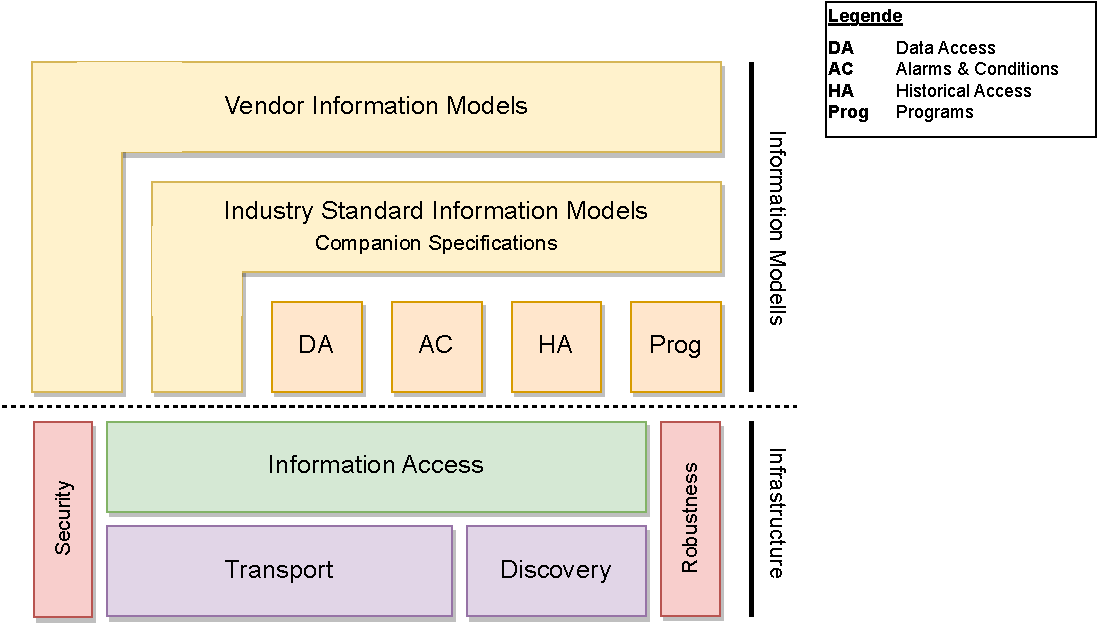
\includegraphics[width=0.9\textwidth]{res/diagramms/companionSpezifikations.pdf}
			\caption{Aufbau des OPC UA Standards, \\ Angelehnt an: Abbildung 1.7 in \cite{mahnke_opc_2009}}
			\label{fig:OPCUA_Framework}
		\end{figure}
	
		\subsection{Kommunikationsaufbau} 
		
		%Client/Server/Field
		OPC UA besteht aus drei Komponenten, deren Zusammenwirkung in Abbildung \ref{fig:OPCUA_Structure} abgebildet ist. Mehrere Field Connections, die die Sensorik oder Maschinen darstellen, mit welchen kommuniziert werden soll. Die Daten sollen zu den OPC UA Clients geleitet werden. Dies können \ac{HMI} oder MES-Systeme sein, die die Daten der Maschinen auswerten oder Steuerungsbefehle absenden möchten. OPC UA standardisiert diese Kommunikation über den OPC UA Server. Dieser setzt den OPC UA Standard um und stellt das notwendige \ac{API} für die Datenabfrage aus der Sicht der Clients zur Verfügung. \cite{rinke_was_2022}
		
		%Integriert oder nicht
		Der OPC UA Server implementiert die proprietären Kommunikationsprotokolle, die vom Maschinenhersteller entwickelt wurden, um mit den Anlagen und den Field Conections zu kommunizieren. Je nach Art der Daten, die die Maschine weiter gibt, werden die Daten auf dem OPC UA Server abgespeichert oder an den Client weiter gegeben. Ein OPC UA Server kann in zwei Formen entstehen. Der Hersteller kann seiner Maschine die OPC UA Standards bereits bei der Entwicklung einprogrammieren. Damit ist der Server in der Maschine integriert und die Maschine ist so von Beginn an OPC UA fähig. Manche SPS Geräte implementieren auch die Möglichkeit einen OPC Server direkt auf der Maschine zu konfigurieren. Sollte der Hersteller die Spezifikationen jedoch nicht implementieren, kann der Server auch zusätzlich zwischen die Maschine und den Client geschallten werden. Durch die Unabhängigkeit des Herstellers sind diese Server oft mit mehr Kommunikationsprotokollen ausgestattet, was deren Möglichkeiten, mit der Maschine zu interagieren erhöht. \cite{rinke_was_2022}
		
		%Pub/Sub
		Die Kommunikation mit dem Client läuft dabei 1 zu 1 ab. Allerdings kann auch ein 1:n Kommunikationsmodell über Publish and Subscribe implementiert werden. Um diese Funktion jedoch zu nutzen, muss der Server mit der OPC UA Pub/Sub Spezifikation erweitert werden. \cite{mielebacher_verteilte_2021}
		
		Der Client kann die Daten über die standardisierte API des OPC UA Servers abfragen. Es können Echtzeitdaten, historische Daten abgerufen werden. Außerdem gibt es eine Spezifikation, wie Alarmierungslogik umgesetzt werden soll. Dies wird anhand der Implementation auf Serverebene deutlich vereinfacht, da sie dann Hersteller unabhängig ist. \cite{rinke_was_2022}
		
		\begin{figure}[H]
			\centering
			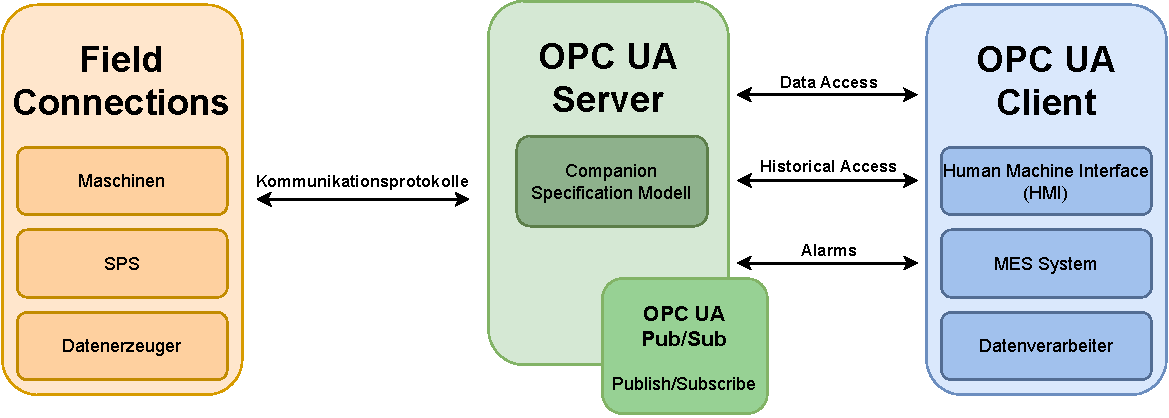
\includegraphics[width=0.9\textwidth]{res/diagramms/OPCUA.pdf}
			\caption{Kommunikationsstruktur OPC UA}
			\label{fig:OPCUA_Structure}
		\end{figure}
		
		In der Automation werden verschiedenste Methoden verwendet, um Endpunkte an eine Anlage anzubinden. In Abbildung \ref{fig:share} sind der Anteil der Verschiedenen Netzwerktypen in der Industrie 2022 veröffentlicht von HMS Networks. Die drei größten Felder sind Fieldbus, Kabellos (Wireless) und Industrielles Ethernet (Industrial Ethernet) wobei letzteres den größte Anteil ausmacht mit 66\%. OPC UA vereint diese Kommunikationsprotokolle in einem Server und so können Clients die Daten über den OPC UA Server auslesen und müssen nicht für jede Maschine ein eigenes Protokoll implementieren. \cite{noauthor_2022_nodate}
		
		Anders Hansson, Chief Marketing Officer von HMS Networks erklärt sich den Wachstum des Industriellen Netzwerkmarktes aufgrund der steigenden nachfrage in der modernen Industrie, nachhaltig, effizient und produktiv zu bleiben und gleichzeitig flexibele und qualitative Fertigung zu ermöglichen. Die Netzwerke zur Kommunikation sind dabei ein Schlüsselfaktor um die genannten Punkte zu erreichen \cite{noauthor_2022_nodate}. Bei einem instgesamten Wachstum der Nutzung dieser Systeme um 8\% zeigen die Entwicklungen in diesen Bereichen eine deutliche Relevanz für die Automatisierung von und Kommunikation mit Maschinen. 
		
		% TODO Vill Kommunikationsprotokolle Analyse Anteile, verwendung AZO
		
		\begin{figure}[H]
			\centering
			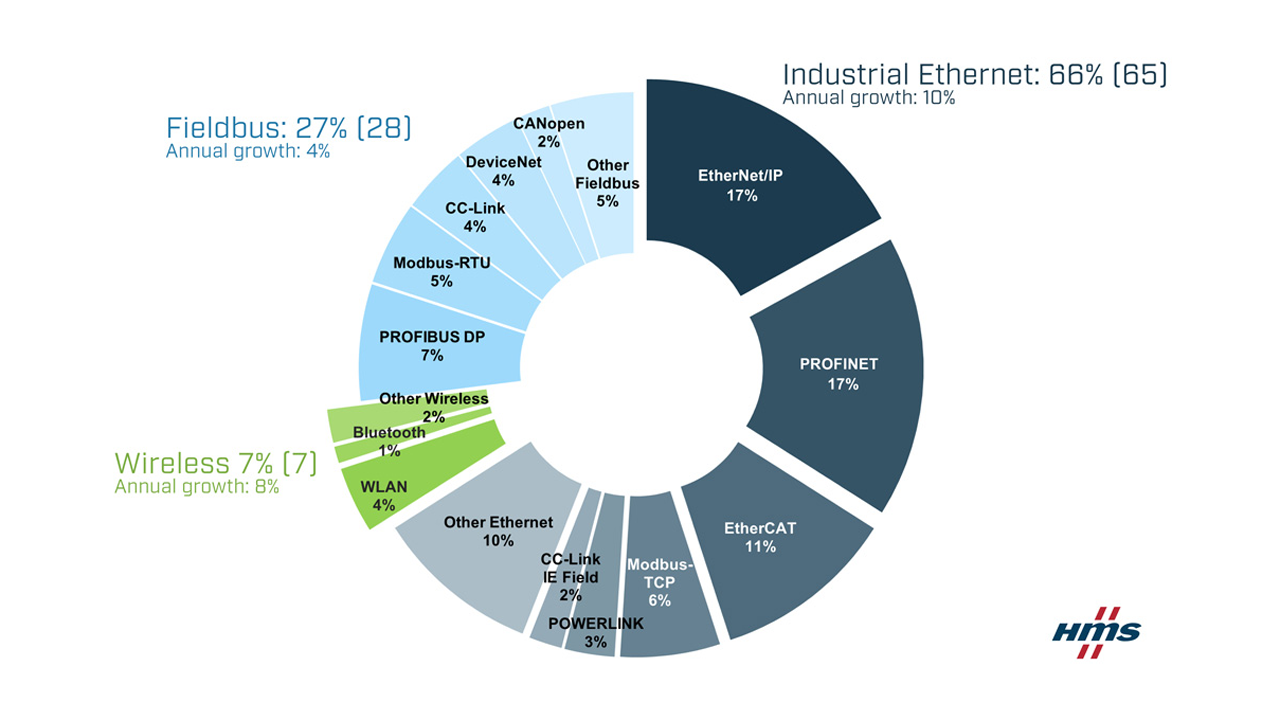
\includegraphics[width=0.9\textwidth]{res/network-shares.png}
			\caption{2022 Industrial network market shares according to HMS Networks \cite{noauthor_2022_nodate}} 
			\label{fig:share}
		\end{figure}
	
		%Nachrichtenaufbau
		OPC UA nutzt einen objektorientierten Ansatz zum Datenaustausch. Dabei werden hierarchische Daten übergeben. Jedes Objekt kann aus Attributen und Methoden bestehen. Die Attribute beinhalten Werte welche gelesen werden können, währen die Methoden vom Client aufgerufen werden können, um der Maschine eine Nachricht zu senden. 
		
		\subsection{Sicherheit}
		
		%Einführung
		Eines der Ziele von OPC UA ist es, eine sichere Verbindung und Kommunikation zu ermöglichen. Die zweite Spezifikation von OPC UA mit dem Titel \glqq Security Modell\grqq definiert die Sicherheit und ist Voraussetzung für die anderen Spezifikationen. Hierin ist festgelegt, welche Sicherheitsmechanismen bei der Nutzung von OPC UA angewendet werden sollen.
		
		% Allgemeines
		Die OPC Foundation beschreibt Unified Architecture mit den Attributen sicher und Firewall freundlich, da OPC UA über den Port 443 kommuniziert, der meist nicht durch Firewalls blockiert wird. OPC UA unterstützt Security auf Transport- und Applikationsebene anhand von selbst entworfenen Protokollen und Erweiterungen von bereits bestehenden Standards. Die Codierung findet auf binärer Ebene statt, wobei die Kommunikation über HTTPS abläuft. Die Authentifizierung von Clients und Servern findet über X509 Zertifikate statt, wobei der Entwickler der UA Anwendung die Anbindung an einen Zertifikatsspeicher selbst übernehmen kann. \cite{noauthor_unified_nodate, noauthor_opc_nodate}
		
		% Authentifizierung/Autorisierung
		Auf Applikationsebene gibt es Sicherheitsmechanismen, welche dir Authentifikation und Autorisierung der Nutzer bearbeiten. Hierbei kommen Passwörtern, Zertifikaten, Webtokens und weiteres zum Einsatz. Außerdem können mit Rechten für Nutzer weitere Einschränkungen auf den Zugriff einzelner Nutzer gelegt werden. Zuzüglich können Aktivitäten von Nutzern und dem System geloggt werden, um die Nachvollziebarkeit zu erhöhen und die Sicherheit des Systems zu stärken. \cite{noauthor_unified_nodate, noauthor_opc_nodate}
		
		%Bundesamt Studie
		Das Bundesamt für Sicherheit in der Informationstechnik führte 2017 eine Sicherheitsanalyse in Kooperation mit TÜV Süd aus und konnte kleine systematischen Fehler in der Sicherheit entdecken. Sie schreiben OPC UA eine hohe Sicherheit zu, wenn die  Mode Sign und security Mode SignAndEncrypt verwendet werden. \cite{damm_opc_2017}
		
		
		%Wenn bei Umati sich etwas ändert, dann dort noch ein Kapitel puschen
	
	\section{\ac{Umati}}
		
		%Einführung
		\ac{Umati} ist eine globale Initiative zur Standardisierung von Schnittstellen zur Kommunikation zwischen Produktionsanlagen. Sie wird vom \ac{VDMA} und dem \ac{VDW} verwaltet, die durch ihre zahlreichen Mitglieder den Standard schnell vorantreiben können. Das Ziel ist es, die Kommunikation zwischen Maschinen möglichst einfach, sicher und einfach zu gestalten. Es soll eine Plug \& Play Umgebung entstehen, in der neue Maschinen in eine Anlage durch bloßes Einstecken ins Kommunikationsnetzwerk integriert werden können. Die \ac{Umati} Initiative entwickelt Standards, welche weltweit zum Einsatz kommen sollen, um eine starke internationale Gemeinschaft um diesen Standard zu erreichen. \cite{noauthor_umati_2023}
		
		%OPC UA in UMATI
		\ac{Umati} baut auf den OPC UA Standards der OPC Foundation auf. OPC UA bildet dabei die Basis und definiert, wie und was kommuniziert werden soll. Es legt fest, was die Rahmenbedingungen für Konnektivität und syntaktische Interoperabilität sind. \cite{noauthor_umati_2023} OPC UA ermöglicht es die semantische Interoperabilität über Companion Spezifications zu versichern. Diese werden auch schon in der Industrie eingesetzt weshalb sich \ac{Umati} die Aufgabe gemacht hat, die verschiedenen Spezifikationen zu vereinheitlichen damit beispielsweise die Identifizierung einer Maschine immer gleich abläuft.
		
		% Automatisierungspyramide
		\ac{Umati} soll vor allem die vertikale und horizontale Integration im Unternehmen erleichtern. In Abbildung \ref{fig:Automatisierungspyramide} ist die Automatisierungspyramide nach Siepmann abgebildet. Je tiefer die Ebene in der Pyramide liegt, desto vielfältiger sind die Systeme dieser Ebene. Während ein Unternehmen nur ein \ac{ERP} System verwendet, kann es zahlreiche SPS und noch mehr Ein- und Ausgabesensoren geben. Diese müssen vertikal integriert werden. Dafür werden Daten von den unteren Ebenen in die Systeme weiter oben zur Verarbeitung überreicht. Bei der horizontalen Integration kommunizieren gleichartige Systeme miteinander. Beispielsweise wenn mehrere SPS Daten austauschen oder Daten Abteilungsübergreifend übergeben werden, wie bei einem Datenfluss von SCM zu CRM System sein. 
		
		\begin{figure}[H]
			\centering
			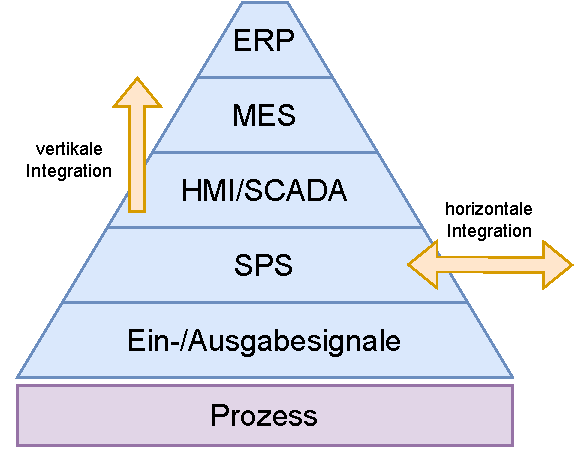
\includegraphics[width=0.8\textwidth]{res/diagramms/Automatisierungspyramide.pdf}
			\caption{Automatisierungspyramide nach Siepmann, \\ Angelehnt an: Folie 8 in \cite{mielebacher_verteilte_2021}} 
			\label{fig:Automatisierungspyramide}
		\end{figure}
		
		\ac{Umati} legt standardisierte Schnittellen fest, mit denen die vertikale und horizontale Integration möglichst einfach umgesetzt wird. Dadurch kann die Wertschöpfung aus Daten kostengünstiger ablaufen und die Analyse, Verarbeitung und Verwertung von Daten, wie es in der Industrie 4.0 üblich ist, besser ablaufen. \ac{Umati} hat bereits Vorführungen auf Messen veranstaltet, welche die Funktionsfähigkeit einer \ac{Umati} Umsetzung demonstrieren. \ac{Umati} standardisiert dabei die Integration von Maschinen, deren Installation und ganze IT Produktionsumgebungen. \cite{noauthor_about_nodate}
		
		% Companion Specifikations
		Die semantische Interoperabilität wurde bereits mit OPC UA über die Companion Spezifikationen erreicht. Allerdings entstehen diese Standards in gesonderten Arbeitsgruppen welche auf die Teilnehmer zugeschnitten sind. Dadurch entstehen viele Spezifikationen in vielen verschiedenen Branchen und Maschinen können nicht mehr ohne Übersetzung kommunizieren. \ac{Umati} versucht diesen Umstand durch das Zusammenfassung dieser Spezifikationen zu beheben. Es sollen Maschinen entstehen, die alle die selbe Sprache sprechen und so einfach in neue IT 
		
		\ac{Umati} selbst besteht aus verschiedenen Modulen, welche alle Standards für verschiedene Bereiche definieren. In Abbildung \ref{fig:OPCUA_for_machinery} sind alle Interfaces abgebildet, welche auf der Base Spezifikation OPC 40001 aufbauen. Dieser wird auch OPC 40001 UA for Machinery genannt und ist für die Anlagenbauindustrie gedacht. \ac{Umati} befindet sich noch in der Entwicklung und ist noch nicht vollständig fertiggestellt, deshalb gibt es Interfaces, welche noch nicht umgesetzt, sondern nur geplant sind. \cite{noauthor_machinery_nodate}
		
		\begin{figure}[H]
			\centering
			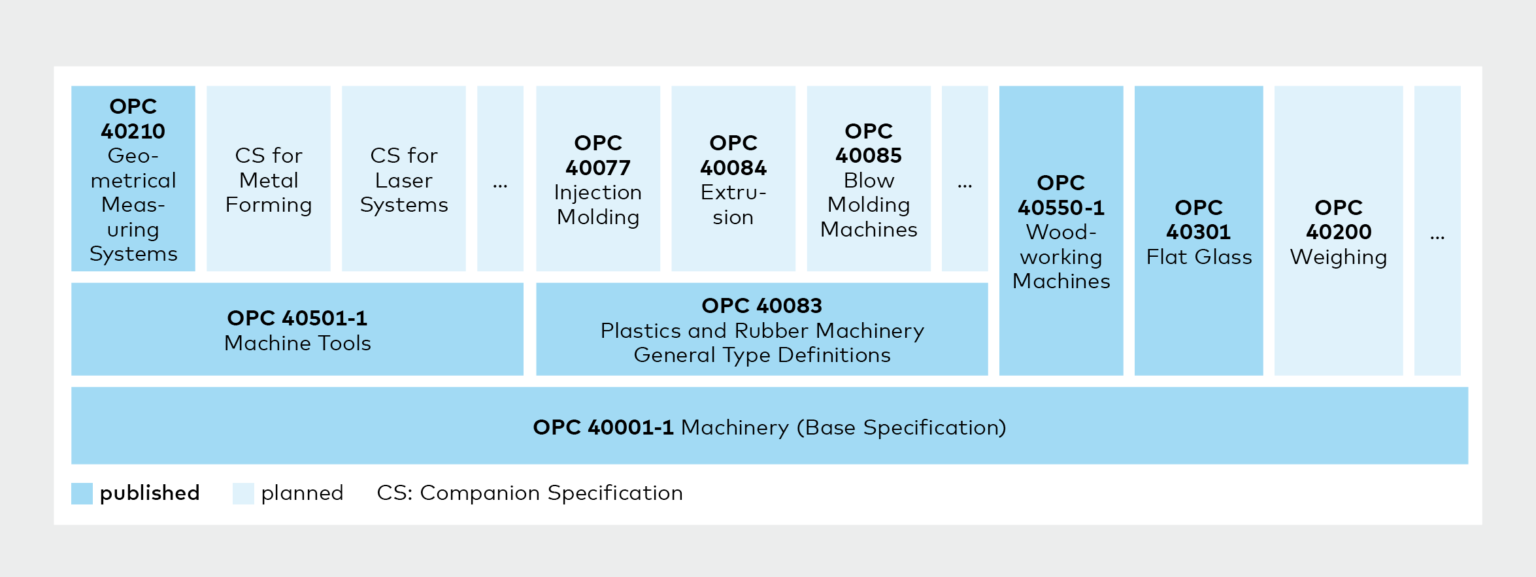
\includegraphics[width=0.9\textwidth]{res/diagramms/OPCUA_for_machinery.png}
			\caption{Interfaces basierend auf OPC UA for Machinery \cite{noauthor_machinery_nodate}} 
			\label{fig:OPCUA_for_machinery}
		\end{figure}
		
		% Kennzahlen, wer nutzt schon, was sind bisherige Meinungen dazu
		
		\subsection{VDMA}
		
		%Allgemin
		\ac{VDMA} ist der größte Industrieverbund in Europa und eines seiner Ziele ist es, \ac{Umati} International zu verbreiten. Der Verband wurde 1892 gegründet und hat seinen Sitz in Frankfurt am Main. Neben der Vertretung der Interessen industrieller Unternehmen in Deutschland und Europa gegenüber der Politik, erarbeitet der VDMA auch Standards und tauscht Know-How zwischen seinen 3.600 Mitgliedsunternehmen aus. \cite{noauthor_verband_nodate} In dem Interessenverband sind Firmen aus den Bereichen Maschinenbau, Anlagenbau und der Zulieferindustrie, welche sich Kompetenzen und Informationen in verschiedensten Themenbereichen von Bildung \& Modernem Arbeiten über Digitalisierung bis zu rechtlichen Feldern teilen. \cite{noauthor_themenubersicht_nodate}
		
		%VDMA Wirken
		Der VDMA wirkt vor allem mit Förderungen in Bereichen, die Innovation bringen. Beispielweise fördert der Verband Technologien in den Bereichen Industrie 4.0, Digitalisierung und nutzt Lobbyarbeit, um seine Mitglieder auch politisch zu unterstützen. Außerdem veranstaltet der VDMA Messen zur Netzwerkbildung und zum Demonstrieren von neusten Technologien seiner Mitglieder. Im Allgemeinen verfolgt der Verband die Stärkung der europäischen Maschinenbaubranche und die Verbesserung der Wettbewerbsfähigkeit auf internationaler Ebene. \cite{noauthor_themenubersicht_nodate}
		
		%AZO
		AZO, der Partner dieser Arbeit, ist auch ein Mitglied des VDMA. Da AZO ein mittelständisches Unternehmen im Anlagenbau ist, setzt sich der VDMA genau für diese Interessen ein und möchte mit \ac{Umati} eine Plug \& Play Umgebung im Anlagenbau ermöglichen. Der VDMA möchte eine erhöhte Interoperabilität zwischen den Maschinen ihrer Mitglieder bewirken und so die Wettbewerbsfähigkeit des europäischen Markts stärken, aber auch in der Standardisierung der internationalen Industrie mitwirken. 
		
		\subsection{OPC UA for Machinery}
		
		\texttt{OPC 40001-1/VDMA 40001-1}, auch OPC UA for Machinery, wurde von VDMA und VDM zusammen mit der OPC Foundation entwickelt. Es ist die fundamentale Spezifikation, auf der andere in diesem Bereich aufbauen sollen. Sie wurde im September 2020 veröffentlicht und seit dem mehrfach aktualisiert worden. Der Standard wird auch in Zukunft erweitert werden, um mehr Use Cases abzudecken. Die neuste Version zum Zeitpunkt des Entwurfs dieser Arbeit ist aus August 2023.
		
		Im Allgemeinen deckt dieser Standard fundamentale Bereiche ab. Es wird definiert, welche Datentypen genutzt werden können, wie deren Syntax ist und wie sie in Attributen abgespeichert werden können. Es werden Objekte und Klassen festgelegt und deren Verhalten und Funktionalität. Darüber hinaus beschreibt die Spezifikation auch, wie ein Client im System die Maschinen an den OPC UA Servern finden kann. 
		
		OPC for Machinery implementiert keinen festen Typ um als einen Einstiegspunkt für den OPC UA Server. Daher muss auf die Basisspezifikation OPC 40001-1 eine weitere Spezifikation aufgesetzt werden. Im Fall dieser Arbeit wird ein Roboter simuliert, weshalb die Spezifikation OPC 40010 Robotics anbietet. Als Mindestanforderung muss Part 1 der Robtics-Spezifikation implementiert werden. Dadurch ergibt sich eine Anzahl an Variablen, Funktionen und Strukturen, welche in den Simulationsserver implementiert werden.
		
		OPC UA for Machinery definiert, das jede Maschine und jede Komponente einen Identifikations-AddIn besitzt. In diesem müssen mindestens eine Manufacturer und eine Productinstance Identifikation vorhanden sein. Dies stellt sicher, dass ein OPC UA Client jede Maschine die Veröffentlicht wird finden und erkennen kann.  

	\section{Weitere Technologien}
		\subsection{Docker}
		
		Docker ist eine Open-Source Virtualisierungstechnologie. Ihr primärer nutzen ist das Anbieten, das Entwickeln und Verwalten von Anwendungen auf einem Serverumfeld. Dabei werden alle Services in eigenen Containern verwaltet, was es ermöglicht einzelne Teile einer Anwendung neu zu starten, sie einfach zu skalieren und einzelne Teile zu beenden, ohne das gesamt System zu beenden. Die Container sind auf die Docker-Engine angewiesen, welche zahlreiche Betriebssysteme unterstützt. Ist eine Anwendung containerized, kann sie auf jeder dieser Betriebssysteme auf Basis einer Docker-Engine gestartet werden. \cite{noauthor_install_2023}
		
		Ein Container wird über ein Docker Image gestartet. Ein Image ist der Bauplan einer Anwendung. In einem Docker Compose File können mehrere Container gestartet werden und deren Startparameter festgelegt werden. Zu diesen Parametert gehören benötigte Ports, Umgebungsvariablen für innerhalb des Containers und welche Version des Images verwendet werden soll. Es können auch virtuelle Netzwerke festgelegt werden, welche die Container auch voneinander abgrenzen. 
		
		Docker hat sich im Bereich der Containersysteme durchgesetzt, da es eine zugängliche Schnittstelle zu dieser Art des Servicedeployment bietet. Docker bietet eine einfache Handhabe und Automatisierte Prozesse zum starten und beenden von Services. Docker Hub trug zum Durchbruch der Virtualisierungslösung ebenfalls bei. Dies ist ein Repository im Internet, in dem zahlreiche Images abgelegt werden können. Die Verwendung von Docker hub erfolgt über einen Nativen Docker Befehl, der das Image herunter läd und zur Nutzung bereitstellt. 
		
		Docker ist die grundlegende Technologie für diese Arbeit. Es wird verwendet um die einzelnen Komponenten des Prototypen zu verbinden. Docker eignet sich durch seine einfache Handhabe und die bereits bestehende Expertise im Unternehmen für die Entwicklung des Prototypen. Auch für die Integration in die AZO Infrastruktur bietet sich Docker an, da bereits eine Dockerumgebung für andere Services besteht. 
		
		\subsection{MQTT}
		
		Das \ac{MQTT} ist eine Nachrichtenprotokoll, dass sich durch seine Robusten Eigenschaften vor allem für unzuverlässige Umgebungen eignet. Es ist entwickelt worden um mit Geräten mit hoher Latenz, geringer Bandbreite oder labilem Netzwerk zu kommunizieren. Es eignet sich vor allem für \ac{M2M}-Kommunikation und den \ac{IoT} Bereich, da es besondere Akku und Leistungssparen ist. 
		
		\ac{MQTT} baut auf einer Subscribe and Publish Architektur auf. Ein Eingabegerät, beispielsweise ein Temperatursensor, erhebt seine Daten und reicht sie an einen MQTT Broker weiter, welcher die Daten veröffentlicht (Publish). Möchte ein Client auf die Daten zugreifen, muss er den korrekten \textit{Topic} unter dem die Daten liegen abonnieren und erhält daraufhin alle Änderungen des Datensatzes (Subscribe).
		
		Der\ac{MQTT} Broker übernimmt das Versenden der Daten an alle Clients. Für einen Client sehen die Topics nach einer hierarchischen Struktur aus. Sollte die Verbindung zu einem Client unterbrochen werden, puffert der Broker die Veränderungen an den Daten und sendet diese, wenn der Client wieder verfügbar ist.
		
		%TODO: \subsection{Grafana}
		%TODO: \subsection{InfluxDB}
		%TODO: \subsection{Telegraf}
		%TODO: \subsection{NodeRed}
		
\chapter{Methodik}\label{ch:Methodiken}
	% (8 Seiten)
	
	% Forschungsmethodik - Deduktiv??? - Konstruktiv???
	
	\section{Literaturrecherche}
	
	Die Informationen der vorangegangenen Kapitel \ref{ch:Einführung} und \ref{ch:Grundlagen} wurden aus offizieller Literatur der Hersteller entnommen. Zu den Informationen zu OPC UA wurden die offiziellen Spezifikationen und empfohlene Literatur der OPC Foundation verwendet. Dasselbe Vorgehen wurde für die theoretische Vorarbeit von \ac{Umati} genutzt. Die meisten Informationen zum neuen Standard wurden der offiziellen Webseite des VDMA entnommen. Zusätzlich wurden die vom VDMA empfohlenen Literaturen für OPC UA und Umati verwendet. Um theoretische Grundlagen und Konzepterklärungen zu recherchieren, wurden Vorlesungsmaterialien der DHBW Mosbach verwendet.
	
	% Datenerhebung - Literaturrecherche
	% Stichwort recherche
	
	% Über die Hersteller empfolene Literatur
	
	\section{Evaluation}
	
	% Evaluation des Ergebnisses
	
	Das Ergebnis dieser Arbeit sind zwei Prototypen zur Demonstration der \ac{Umati} Spezifikation. Diese Prototypen werden anhand bestimmter Kriterien bewertet, welche aus dem Standard ISO 25010 für Softwarequalität entnommen wurden. In Abbildung \ref{fig:ISO25010} sind die Softwarequalitätskriterien strukturiert abgebildet, wie sie im ISO-Standard definiert sind. 
	
	\begin{figure}[H]
		\centering
		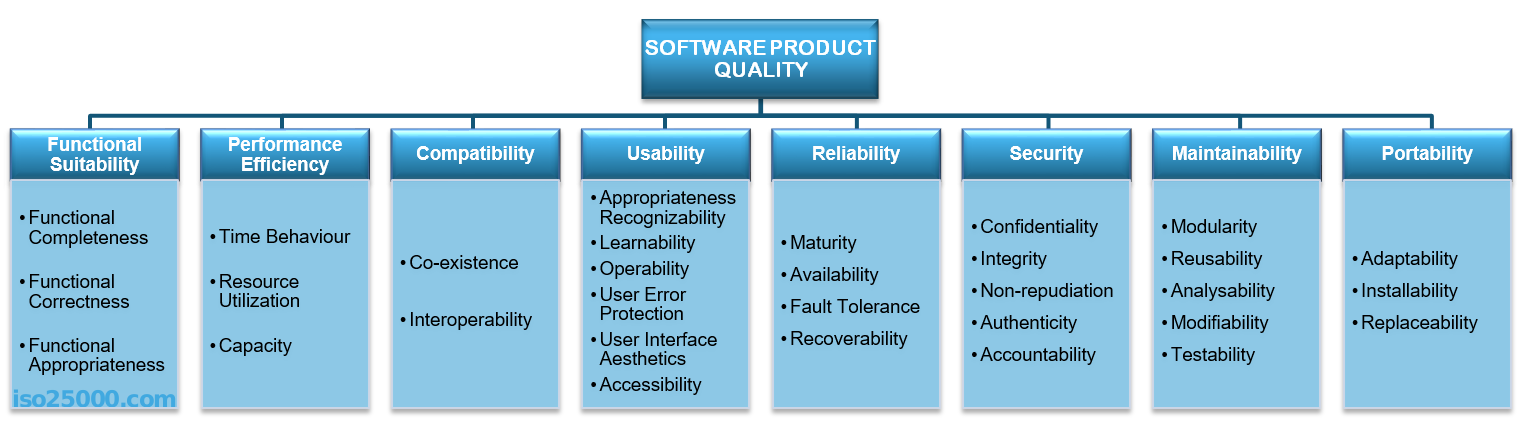
\includegraphics[width=0.9\textwidth]{res/diagramms/iso25010.png}
		\caption{Softwarebewertungskriterien ISO 25010} 
		\label{fig:ISO25010}
	\end{figure}
	
	Die Punkte \textit{Functional Suitability}, \textit{Performance Efficiency}, \textit{Usability} und \textit{Reliability} sind die Hauptkriterien die für die Messeprototypen besonders wichtig sind. Die anderen Kriterien sind ebenfalls von Wichtigkeit, können jedoch den anderen nachgestellt werden, da die Prototypen nur demonstrativen Nutzen hat. 
	% TODO: Warum???
	% TODO: Quantifizierbare Ziele setzen
	
	Das Demomaterial welches für die Messe ausgelegt werden soll, muss visuell anschaulich sein und die Kernfunktionen von \ac{Umati} präsentieren. Es geht darum das Interesse der Messebesucher zu wecken und genug Informationen für ein allgemeines Bild über die Funktionen und Ziele von \ac{Umati} zu erreichen. 
	
	%TODO: Reflexion
	% Evaluation der Prototypen
	
	\section{Zeitplanung}
	
	Die Bearbeitungszeit dieser Arbeit beträgt zwölf Wochen, von Montag dem 19.06.2023 bis Montag den 11.09.2023. In Abbildung \ref{fig:Grantt} ist ein Grantt-Diagramm der Zeitplanung abgebildet. In den ersten 4 Wochen sollen die Theoretische Grundlagen und die Analysen der Arbeit abgeschlossen sein, damit die Praxis am 10.07.2023 beginnen kann. Von Woche 5 bis 10 soll die Implementation und Integration der Prototypen stattfinden. Der gesamte Prozess kann auf gemeinsam 5 Wochen geschätzt werden, wobei eine zusätzliche Woche als Puffer eingeplant wird, sollte es Verzögerungen wie Krankheit oder Bereitstellungsschwierigkeiten geben. Am 21.08.2023 soll die Arbeit abgabebereit sein und für eine Korrekturlesung bereitgestellt werden. Parallel zur Korrekturlesung sollen die Messedokumente und Schulungsunterlagen angefertigt werden. Der letzte Block dient als Puffer für den Abschluss der Arbeit.
	
	\begin{figure}[H]
		\centering
		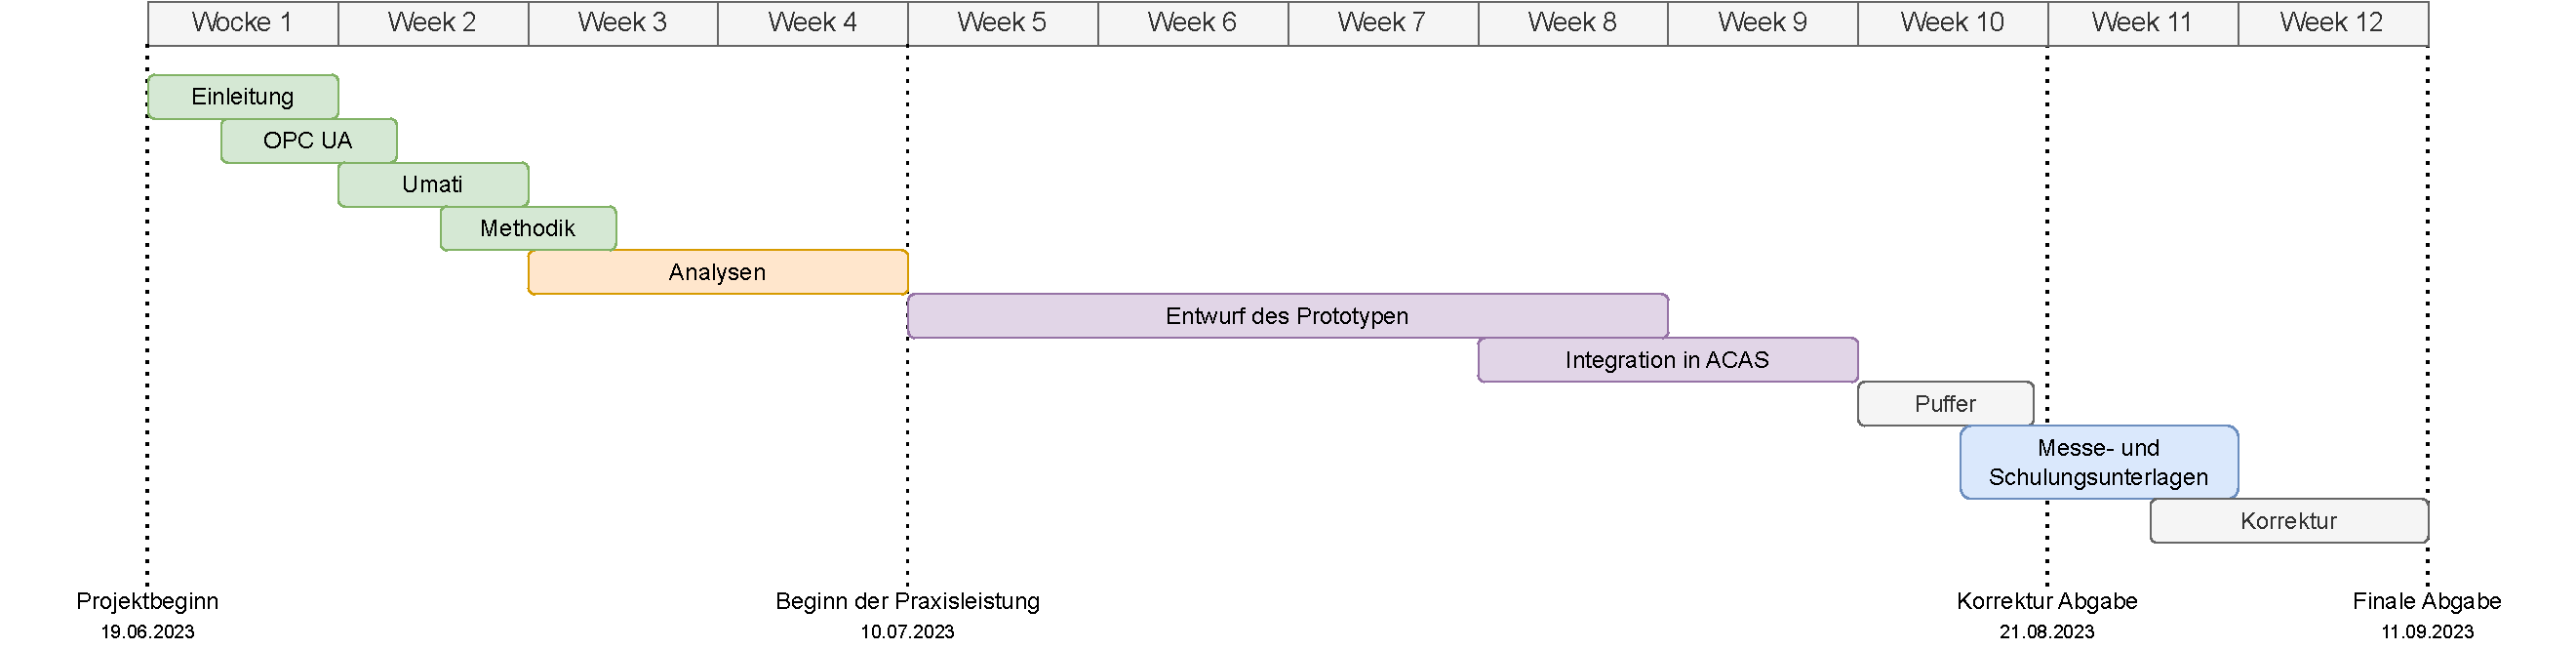
\includegraphics[width=0.9\textwidth]{res/analysen/Grantt-Diagramm.pdf}
		\caption{Grantt-Diagramm zum Projektablauf}
		\label{fig:Grantt}
	\end{figure}
	
	Der Zeitplan erwies sich als hilfreich, zur Bewertung des momentanen Fortschrittes der Arbeit. Die Ausarbeitung der Einfleitung und Grundlagen verliefen nach Zeitplan. Dadurch war das Projekt nach Woche 4 im Zeitplan und das Praxisprojekt konnte rechtzeitig gestartet werden. Durch Verzögerungen bei der Entwicklung des OPC UA Servers und der Entscheidungsfindung, welcher Verwendet werden sollte, schob sich jedoch die Implementationsphase in den Puffer hinein. Dank des Puffers konnte die Arbeit jedoch dennoch Zeitgerecht bis zur Korrekturabgabe fertiggestellt Werden. Die letzten Arbeitspakete konnten ebenfalls vor der finalen Abgabe fertiggestellt werden.  
	
\chapter{Ergebnisse}\label{ch:Ergebnisse}
	
	% (8 Seiten)
	
	\section{Anforderungsanalyse}
		
		\subsection{Vorgehen}
		%Ziel
		Das Ziel dieses Projekts ist es, die Umsetzbarkeit eines umatifähigen OPC UA Servers zu demonstrieren. Es sollen Daten von einer Maschine ausgelesen und angezeigt werden. Es soll eine Struktur entworfen werden, welche den Datenfluss von OPC UA Server an eine Visualisierungsoberfläche ermöglicht.
		
		Zunächst soll der erste Prototyp umgesetzt werden, bei welchem Daten an die offizielle Webseite des VDMAs gesendet werden sollen. Diese Webseite demonstriert, dass verschiedenste Hersteller auf einem gemeinsamen Dashboard ihre Maschinen und Anlagen mit Umati integrieren können. AZO möchte eine eigene Maschine dort anzeigen, welche auf Messen gezeigt werden kann.
		
		Der zweite Prototyp ist eine Verbindung zwischen einem OPC UA Server mit der Umati Implementation und einer internen Visualisierung. Hierbei sollen die Daten aus dem OPC UA Server ausgelesen und so transformiert werden, dass sie auf einem Grafana Dashboard angezeigt werden können. AZO visualisiert bereits bestehende Projekte über Grafana und die Umati Maschinen sollen sich so in die bereits bestehende Infrastruktur eingliedern.
		
		\subsection{Prototyp 1: Umati Web Dashboard}
		
		% Ziel
		Die Daten eines OPC UA Servers sollen an das Umati Web Dashboard gesendet werden. Die Seite kann unter dem Link \textit{umati.app} erreicht werden. Sie baut auf einem MQTT Broker auf, welcher alle Daten der Teilnehmer abspeichert und an das Dashboard weiter gibt. Der MQTT Broker liegt an derselben Adresse am Port 443 und benötigt Anmeldekriterien für die Veröffentlichung und das Abfragen von Daten.
		
		% Prototyp
		Als Grundlage des ersten Prototyps soll eine Maschine simuliert werden. Es soll keine echte Maschine verwendet werden, da diese eventuell an bestimmten Zeitpunkten ausgeschaltet oder betriebsunfähig sein könnte. Außerdem ist eine laufende Maschine oder Anlage deutlich kostenintensiver als eine serverbasierte Simulation. Die simulierte Maschine soll eine Anlage von AZO darstellen, die auch tatsächlich im Einsatz ist. Als Beispiel wird ein RoLog simuliert, der bei der automatischen Kleinstmengendosierung von Schüttgütern zum Einsatz kommt. In Abbildung \ref{fig:RoLog} ist ein virtualisierter Aufbau der Anlage abgebildet. Der Roboterarm in der Mitte lagert seine Ressourcenbehälter auf den Schränken an der Seite der Anlage, lagert neue Behälter über die Laufbänder an der Hinterseite (Oben-Links) aus oder ein und dosiert in die Ausgabe an der Front (Vorne-Rechts) des Aufbaus. \cite{noauthor_azo_nodate}
		
		\begin{figure}[H]
			\centering
			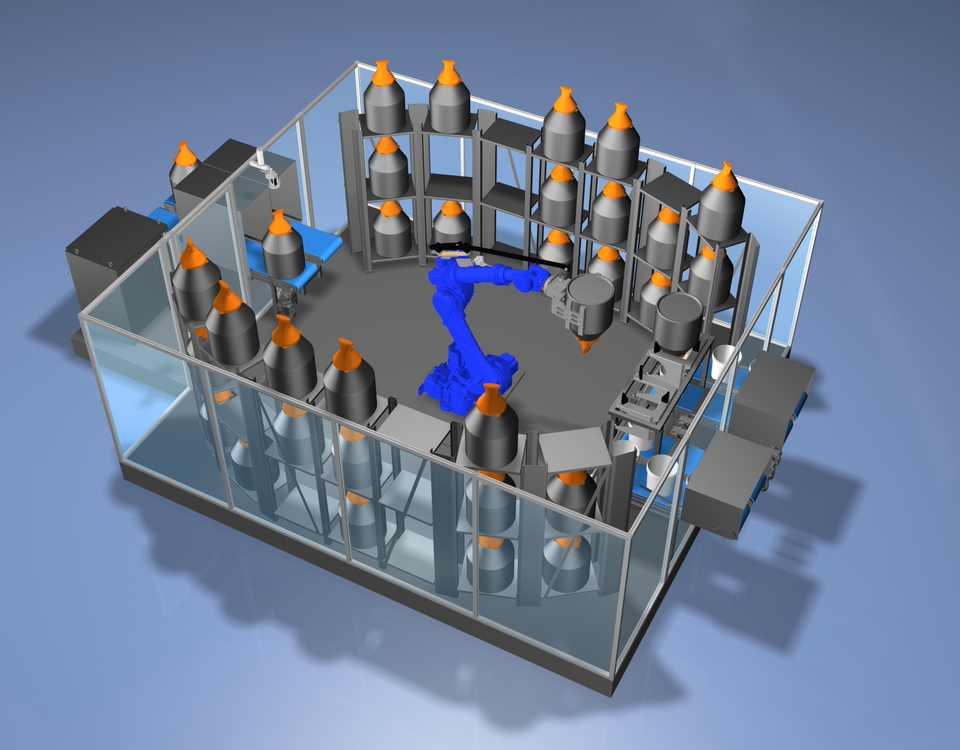
\includegraphics[width=0.7\textwidth]{res/RoLog.png}
			\caption{RoLog von AZO Gmbh \& Co. KG \cite{noauthor_azo_nodate}}
			\label{fig:RoLog}
		\end{figure}
	
		Der erste Prototyp hat mehrere Kriterien, die erreicht werden müssen. Folgende Anforderungen wurden für den ersten Prototyp erstellt:
		
		% Evaluationskriterien
		\begin{itemize}
			\item \textbf{REQ1}: Kommunikation von OPC UA Server zu Client nach Umati Standard
			\item \textbf{REQ2}: Daten auf Umati Web-Dashboard:
			\subitem \textbf{REQ2.1}: Visualisierung der Daten, die sich verändern.
			\subitem \textbf{REQ2.2}: Personalisieren aller Daten nach AZO Gmbh.
			\subitem \textbf{REQ2.3}: Anpassen der Location auf der Karte.
			\subitem \textbf{REQ2.3}: Anzeige eines Bild der Maschine.
		\end{itemize}
		
		\subsection{Prototyp 1: Umati Web Dashboard}
		
		% Ziel
		Die Daten, welche die Simulation der Maschine generiert, sollen an eine Grafana Instanz gesendet werden. Hier soll erneut ein umatifähiger OPC UA Server verwendet werden. Die Daten sollen in der grafischen Oberfläche von Grafana einfach und umfangreich ausgelesen und angezeigt werden können. Das Ziel ist es, einen Ablauf zu entwerfen, welcher als Ansatzpunkt für zukünftige Projekte verwendet werden kann. 
		
		% Grafana
		Grafana soll dabei in einem Docker-Container laufen. Grafana bietet Nativ die Möglichkeit, unterschiedliche Datenquellen einzubinden. Eine dieser Datenquellen soll verwendet werden. Es soll ein Dashboard entstehen, welches die Daten der Maschine anzeigt und sich live aktualisiert. Aus den Ansätzen folgern diese Anforderungen:
		
		% Evaluierungskriterien
		\begin{itemize}
			\item \textbf{REQ1}: Kommunikation von OPC UA Server zu Client nach Umati Standard
			\item \textbf{REQ2}: Grafan muss in einer Docker Instanz laufen.
			\item \textbf{REQ3}: Dashboard:
			\subitem \textbf{REQ3.1}: Visualisierung der Daten, die sich verändern.
			\subitem \textbf{REQ3.2}: Einbinden einer Datenquelle, die Grafana Nativ versteht.
			\item \textbf{REQ4}: NodeRed soll als Lösung in Betracht gezogen werden.
		\end{itemize}			
		
	\section{Lösungsansatz}
	
		\subsection{Grundlagen}
		% OPC 40001 for Machinery
		Der OPC UA Server muss mehrere Spezifikationen implementieren. Als Grundlage muss die Identifikation der Maschinen aus der OPC 40001 for Machinery Spezifikation genutzt werden. Der OPC UA Server erstellt dabei einen Namespace, in dem alle Anlagen einem Ordner mit der Bezeichnung \textit{Machines} untergeordnet sind. Jede Komponente und jede Maschine müssen einen Identifikations-Ordner besitzen. Dieser Ordner ermöglicht es, dass OPC UA Clients alle Maschinen finden und sie richtig erkennen. 
		
		% OPC 40010 Robotics
		Da die Basisspezifikation jedoch keinen eigenen Einstiegspunkt definiert, muss eine weitere Spezifikation implementiert werden. Diese Arbeit wird die OPC 40010 Robotics - Vertical Integration Spezifikation implementieren. Diese legt fest, welche Komponenten in welcher Art und Weise vorhanden sein müssen, um eine Maschine im Roboticsumfeld mit Umati zu betreiben. Es muss ein \textit{MotionDeviceSystem}, ein \textit{Robot} und ein \textit{RobotController} existieren. 
		
		% Mandatory Objects
		Der \textit{Robot} implementiert die Achsen und Motoren der Maschine und hat ein Attribut mit den Werten der Geschwindigkeit, Beschleunigung und Position. Der \textit{RobotController} verwaltet das \textit{Robot}-Objekt und speichert noch zusätzliche Informationen ab. Beispielsweise welche Software verwendet wird, um den Roboter zu steuern und einige Sicherheitsfeatures. Die \textit{MotionDeviceSystem} verwaltet die \textit{RobotController} und stellt die Anlage im ganzen dar.
		
		% Aufbau VM
		Die gesamte Infrastruktur des Projektes wird auf einer VM mit Ubuntu Server 20.04.2 laufen. Auf der VM ist die Docker Engine installiert. Um die Vorgänge auf dem Server besser nachvollziehen zu können, ist eine Portainer Instanz als Docker Container installiert. Portainer ist eine grafische Oberfläche, die über den Browser erreicht werden kann. Sie ermöglicht den Umgang mit Docker Containern, Images und allem was Docker zur Verfügung stellt sehr einfach. Unter anderem kann eine Konsole innerhalb der Container gestartet werden, was die Entwicklung extrem vereinfacht. 
		
		\subsection{OPC UA Server}
		
			\subsubsection{OPC UA Server - DataFeed}
				
			Die Softing Industrial Automation GmbH bietet zahlreiche Tools an, um mit OPC UA Servern zu Kommunizieren und auch diese zu entwickeln. Sie bieten unter dem Namen dataFEED OPC Suite Base ein Produkt an, welches die Kommunikation mit OPC UA und OPC Classic und die Cloud-Anbindungen übernimmt. Dabei ermöglichen sie die Kommunikation mit führenden Herstellern von Steuerungen wie  Siemens SIMATIC S7, Rockwell ControlLogix, B\&R, Mitsubishi sowie auf Modbus-Steuerungen. \cite{noauthor_datafeed_nodate}
		
			Bei AZO wird diese Suite verwendet, weshalb die Implementierung eines OPC UA Servers mit Umati über dataFEED infrage kam. Allerdings lässt der Baukasten zum Entwurf der OPC UA Server keine Objekte zu, welche notwendig sind, um Umati zu implementieren.
					
			\subsubsection{Eigenimplementierung}
		
			% Eigenimplementierung in LowCode Plattform NodeRed
			% Muss ich noch rechachieren
					
			Da der Umati Server auf dem offenen Standard OPC UA aufbaut, kann ein Server auch selbst implementiert werden. Dies hat verschiedene Vor- und Nachteile, welche beachtet und auf das Ziel der Implementierung angewandt werden müssen. 
			
			Eigenimplementierungen sind meist anpassungsfähiger und flexibler, um auf Situationsspezifische Anforderungen zu reagieren. Sie können spezifisch auf den gewünschten Zweck hin optimiert und verbessert werden. Dies kann auch eine einfachere Integration in eine bereits bestehende Umgebung garantieren, da die Anwendung auf diese Umgebung hin angepasst werden kann.
			
			Allerdings kann es auch zu Nachteilen führen. Eigenimplementationen haben ein hohes Risiko auf Fehleranfälligkeiten oder Sicherheitslücken. Bei eingekauften Lösungen profitiert die Anwendung im Normalfall von Erfahrungswerten des Breitstellers und dem Umstand, dass diese Lösung sich bereits am Markt behaupten musste. Die fehlende Erfahrung kann auch zu einem Programm führen, welches kaum optimiert und komplex ist, was die Wartbarkeit und Nutzerfreundlichkeit vermindert. Soll die Lösung zu kommerziellen Zwecken eingesetzt werden oder hat hohe Anforderungen an Sicherheit, Zugverlässlichkeit und Robustheit, sollte auf eine Eigenimplementation verzichtet werden.
			
			Trotz der Nachteile sollte die Umsetzung einer Eigenimplementierung, vor allem zu Demonstrationszwecken, in Betracht gezogen werden. Hierbei gibt es Low-Code und High-Code Ansätze. Bei High-Code Implementierungen wird die Funktionalität in Code hergestellt. Beispielsweise kann ein OPC UA Server nur anhand von Python oder C\# Frameworks implementiert werden. Low-Code Ansätze bedienen sich dabei einem visuellen Programmierstil. Die Programmierung findet über IDEs statt, welche mehr auf Bausteinartige Programmierung setzen. Beispiele für solche Umgebungen sind NodeRed oder Microsoft Power Apps. 
			
			\paragraph{Implementierung mit C\#}
			Die OPC Foundation stellt ein Framework für die Entwicklung von OPC Servern auf C\# Basis zu Verfügung. Die OPC UA.NET Standard-Bibliothek ermöglicht die Entwicklung von OPC Servern und Clients. Eine Eigenimplementierung mit diesem Framework würde einen sehr individualisierbaren und flexiblen Server ergeben, welcher den RoLog in seiner exakten Funktion darstellen könnte. Allerdings ist die Implementierung sehr zeitintensiv und benötigt Expertise auf dem Bereich. \cite{noauthor_opc_nodate-1}
			
			Um eine einwandfreie Simulation eines RoLogs als Basis der Prototypen zu verwenden, sollte diese Implementierung in Betracht gezogen werden. Allerdings ist diese Form, um einen ersten \ac{PoC} für Umati zu entwerfen, zu aufwendig.
			
			\paragraph{Implementierung in einer SPS}
			Die Implementierung einer OPC UA Schnittstelle kann auch direkt auf einer SPS durchgeführt werden. Siemens SPS stellen einen integrierten OPC UA Server zu Verfügung, welcher direkt an der Anlage laufen kann. Es gibt auch die Möglichkeit, Maschinen zu simulieren und mit kleinen Programmen deren Verhalten zu bestimmen. Der Server der SIMATIC S7 SPS von Simens kann Objekte und Klassenstrukturen darstellen. \cite{noauthor_tia_2019}
			
			Die Entwicklung eines solchen Servers ist sehr zeitaufwendig und benötigt Expertise im Entwickeln von OPC UA Servern auf SPS. Es ist denkbar Maschinen die umatifähig sein sollen, auf dieser Ebene als OPC UA Server zu entwickeln, allerdings für eine Demonstration von Umati zu Umfangreich.
			
			\subsubsection{Vorgefertigte OPC UA Server mit Umati}
			
			Es können ebenfalls bereits vorhandene OPC UA Server verwendet werden. Da Umati als Kommunikationsstandard noch sehr jung ist und sich noch nicht Weltweit durchgesetzt hat, gibt es nur wenige Implementierungen. Allerdings bietet der VDMA eigene Implementierungen auf deren GitHub an. Dort können mehrere Implementierungen von OPC UA Servern mit Umati Spezifikationen gefunden werden. In Kapitel \ref{Marktanalyse} wird auf die Repositories des VDMAs genauer eingegangen.
	
	\section{Marktanalyse}\label{Marktanalyse}
		
		Die Initiatoren von Umati, der \ac{VDMA} und \ac{VDW}, stellen mehrere GitHub Repositorien mit vorgefertigten Projekten zum Thema Umati zur Verfügung \cite{noauthor_github_nodate}. All diese Projekte sind unter dem Namen \textit{umati - universal machine technology interface} zusammengefasst. Hier finden sich auch mehrere Sample Server und Implementierungen von OPC UA Servern in verschiedenen Sprachen. Zum Zeitpunkt dieser Arbeit am 23.08.2023 sind 18 Repositorien in diesem Verzeichnis aufgeführt. Eine davon enthält ein Tutorial zum Erstellen eines Servers für einen Showcase (https://github.com/umati/Showcase). Hier können alle Informationen entnommen werden, die für den Prototyp 1 - Umati Web Dashboard benötigt werden.
		
		Das Repository Verzeichnis enthält drei Implementierungen von Sample-Servern, welche in Rahmen dieser Arbeit genauer betrachtet wurden. Der \textit{Sample-Server} \linebreak (https://github.com/umati/Sample-Server) ist eine Implementierung mit Maschinensimulation auf Basis von C++. Er implementiert die Companion-Spezifikationen OPC UA Machine Tool, OPC UA for Woodworking, OPC UA for Geometrical Measuring Systems und OPC UA for Additive Manufacturing. Da die Robotics Spezifikation für diesen Server noch Work-In-Progress ist, muss ein anderer verwendet werden.
		\% Datenfluss -> Bildbeschreibung
		Ein anderer Server auf Basis des Python-Frameworks asyncio (https://github.com/umati/Sample-Server-asyncio) implementiert die Companion Spezifikationen OPC UA Plastic and Rubber, OPC UA for Woodworking, OPC 40451–1 Tightening und OPC UA for Surface Technology. Auch in diesem Projekt ist die Robotics Spezifikation noch nicht implementiert.
		
		Nach Rücksprache mit Götz Görisch vom VDMA fiel die Entscheidung, welchen Sample Server verwendet werden soll, auf den \textit{Sample-Server-node-opcua}. Dieser OPC UA Server ist mit TypeScript programmiert und hat neben vielen weiteren auch die Robotics Companion-Spezifikation implementiert. Da sich dieser Server in einem Dockercontainer starten lässt und bereits alle notwendigen Entrypoints für einen Roboter vorhanden sind, wurde dieser Sample-Server für das Projekt verwendet.
		
		Für den OPC UA Client stellt der VDMA ebenfalls ein Repository zur Verfügung. Der \textit{Dashboard-OPCUA-Client} (https://github.com/umati/Dashboard-OPCUA-Client) übernimmt die Verbindung zwischen dem OPC UA Server und einem MQTT Broker. Der Container des OPC UA Clients des VDMAs benötigt zum Starten eine configuration.json, in der die Adressen zum OPC UA Server und dem MQTT Broker stehen. Außerdem beinhaltet diese Datei, welche Companion Spezifikationen im angegebenen Namespace gefunden werden sollen. 
		
	%\section{Wirtschaftlichkeit und Projektanalyse}
	
		%\subsection{Kostenplanung}
		
		%\subsection{Fallbeispiel}
			% Beispielswiese an Fallbeispiel -> Durchschnittliche AZO Straße
			% -> Probleme bei Schnittstellen integrierung.
	
\chapter{Implementierung}\label{ch:Implementierung}
	
	\section{Veröffentlichung von Daten auf dem Umati Web-Dashboard}\label{ch:Implementierung-Web}
		
		% Ziel und Motivation
		Das Umati Web-Dashboard ist ein Projekt des VDMAs welches die Funktionalität zur Datenabfrage an Maschinen durch Umati demonstrieren soll. Mitglieder des VDMAs und Interessenten an Umati können eigene Maschinen umatifähig machen und sie für Ausstellungszwecke auf diesem Web-Dashboard anzeigen lassen. AZO möchte ebenfalls eine eigene Maschine auf diesem Dashboard anzeigen lassen. Dies soll vor allem für Messezwecke umgesetzt werden, aber auch um die grundlegenden Funktionen von Umati zu erforschen.
		
		In Abbildung \ref{fig:umatiApp} ist das Ziel der Anzeige abgebildet. Die uamti.app besteht aus einer Hauptseite, auf der Maschinen von verschiedenen Herstellern auf einer geografischen Karte markiert sind. Diese Markierungen können angeklickt werden, um weitere Informationen über die Maschine auszugeben. In Abbildung \ref{fig:umatiApp} ist der ausgewählte RoLog abgebildet. Nach Bedarf kann auf eine Detailansicht navigiert werden, welche die Variablen, Parameter und Eigenschaften der Maschine anzeigt.
		
		\begin{figure}[H]
			\centering
			\includegraphics[width=0.9\textwidth]{res/UmatiApp.png}
			\caption{Anzeige des RoLog Controllers auf dem Umati Web-Dashboard}
			\label{fig:umatiApp}
		\end{figure}
		
		\subsection{Struktur}
		
		% Verwendete Komponenten
		Die Struktur des ersten Prototyps besteht aus zwei Docker-Containeren. Der RoLog ist ein modifizierter Container des \textit{Sample-Server-node-opcua} von Andreas Heine, welcher einen OPC UA Server veröffentlicht, der Umati implementiert. Dieser Daten werden vom OPC UA Client ausgelesen. Dieser basiert auf dem Container aus dem \textit{Dashboard-OPCUA-Client} Repository. Der OPC UA Client sendet die Daten weiter an einen MQTT Broker. Dieser kann unter der Adresse \textit{https://umati.app:443/} erreicht werden und veröffentlicht die gesendeten Daten zur Abfrage. Das Frontend des Dashboards synchronisiert sich daraufhin mit dem MQTT Broker, erhält die Daten und zeigt sie auf der Webseite an. In Abbildung \ref{fig:Prototyp1} ist der Aufbau illustriert. Um zu überprüfen, ob die Daten auch tatsächlich auf dem MQTT Broker ankommen, kann mit einem MQTT Client auf den Broker zugegriffen werden und die Daten ausgelesen werden.
		
		\begin{figure}[H]
			\centering
			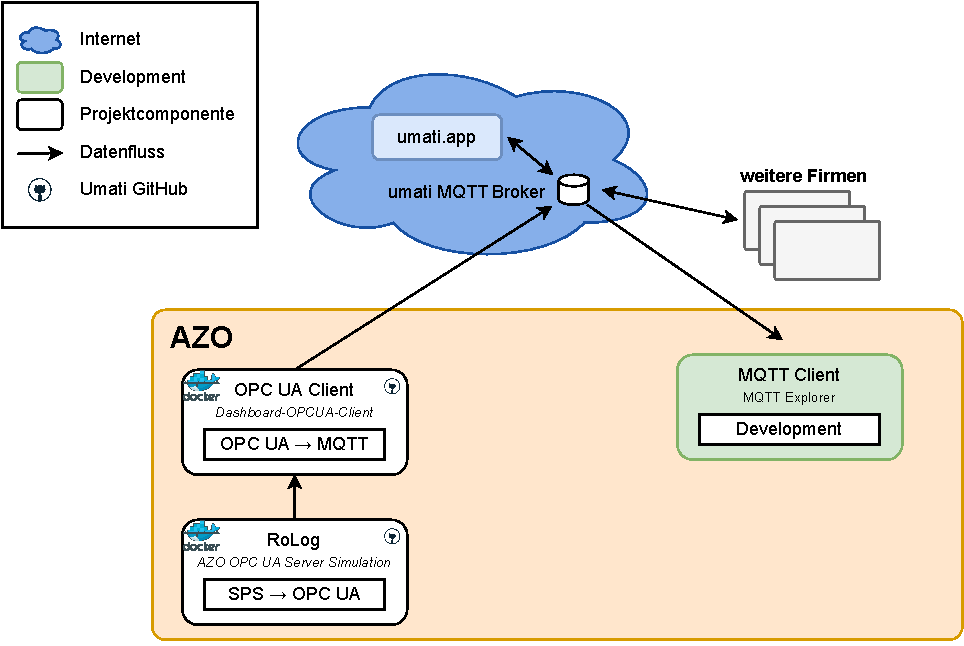
\includegraphics[width=0.9\textwidth]{res/implementierung/Prototyp-umatiWeb.pdf}
			\caption{Struktur des ersten Prototypen}
			\label{fig:Prototyp1}
		\end{figure}
		
		% Requirements - Anmeldedaten
		Um die Daten auf das Umati Web-Dashboard zu senden, werden mehrere Dinge benötigt. Anmeldedaten um mit dem MQTT Broker zu kommunizieren und es muss eine \ac{MoU} unterschrieben werden. Dafür muss eine E-Mail an \textit{info@umati.org} gesendet werden, mit einer Beschreibung der Maschine, die angebunden werden soll. 
		
		\subsection{RoLog OPC UA Server}\label{ch:RoLogOPCUA}
		
		% Source
		Der OPC UA Server mit simulierter Maschine ist aus dem Repository \textit{Sample-Server-node-opcua} des VDMAs entstanden. Um das Projekt anzupassen, wurde ein Fork des Repositories erstellt und lokal abgespeichert. Der Server beinhaltet mehrere simulierte Maschinen, die der OPC UA Client später ignorieren wird, weshalb nur die für die OPC for Robotics Spezifikation relevanten Maschinen angepasst werden müssen. 
		
		% Konfiguration Simulation
		Die Konfiguration der Maschinen findet in XML Dateien statt. Diese liegen im Projekt unter dem Ordner mit der Bezeichnung \textit{models} ab. Alle benötigten Maschinen werden in der \textit{opcroboticstestserver.xml} definiert. Folgende Parameter können angepasst werden:
		
		\begin{itemize}
			\item \textbf{Location} an drei Stellen sollte auf die Position der Maschine geändert werden. ("N 49.4439397 E 9.4087658")
			\item Die Bezeichnung der Maschinen sollte geändert werden.
			\subitem Die \textbf{ManufacturerUri} Eigenschaft sollte geändert werden.
			\subitem Die \textbf{ComponentName} Eigenschaft kann angepasst werden. 
		\end{itemize}
		Jede Eigenschaft hat einen Value Abschnitt, in den ein personalisierter Wert eingetragen werden kann.
		
		% Docker Compose
		Nach der Anpassung der XML-Datei kann ein Dockercontainer erstellt werden, in dem der Server läuft. Um nicht bei jedem neu starten des Containers alle Startparameter erneut an den Befehl anheften zu müssen, wird eine Docker-Compose Datei erstellt, die diese Parameter enthält. Die folgende Docker-Compose Datei startet den OPC UA Server.
		
		\lstinputlisting[frame=single]{res/code/compose-rolog.yaml}
		
		% Starten des Docker Containers
		Diese Docker-Compose Datei startet einen Container mit dem Namen \textit{opcua-rolog} aus dem Ordner in dem sie abgespeichert ist. Diese Datei muss im selben Ordner wie das Dockerfile des Forks für den Sample Server liegen. Es verbindet den Port 4840 des Hostsystems mit dem Port 4840 des Containers. Wird nun eine Anfrage an den Port des Hostsystems gesendet, reicht dieser sie an den Port des Containers weiter. Dieser Port kann auch eine anderer sein, sollte 4840 bereits belegt sein (Beispiel: "4841:4840", um den Port 4841 des Hostsystems zu verwenden). Der Container kann mit einem Docker Compose Befehl gestartet werden. 
	
		\begin{lstlisting}[numbers=none, language=bash, frame=single]
			docker-compose -f docker-compose.yaml up --build -d
		\end{lstlisting}
	
		% Docker Befehl Beschreibung - Logs
		Der Befehl führt die Docker-Compose Datei mit dem Namen \textit{docker-compose.yaml} aus, dank der \textbf{-f} Flag. Durch \textbf{--build} wird der Container bei jedem Ausführen des Befehls neu erstellt, um sicherzustellen, dass alle Veränderungen an den Quelldateien auch im Container verwendet werden. Die Detached Flag \textbf{-d} gibt die Konsole nach dem Starten des Containers wieder frei. Fehlt diese Flag, bleibt die Konsole in den Logs des Containers. Um im Nachhinein auf die Logs des Containers zugreifen zu können, kann folgender Befehl verwendet werden. 
		
		\begin{lstlisting}[numbers=none, language=bash, frame=single]
			docker logs [Container] --follow
		\end{lstlisting}
		
		% Docker Befehl beschribung
		\textit{[Container]} muss durch den Container Namen oder die ID des Containers ausgetauscht werden. Das \textbf{--follow} bewirkt, dass die Konsole im Logging Modus bleibt und nicht nach der letzten Ausgabe den Container wieder verlässt. Um den Logging Modus zu verlassen, kann die Tastenkombination Strg + C verwendet werden.
		
		% Überprüfung 
		Um zu überprüfen, ob der Server die richtigen Daten veröffentlicht, kann ein OPC UA Client verwendet werden. UAExpert bietet eine grafische Oberfläche an, über die durch alle Objekte des OPC Servers gesucht werden kann. In Abbildung \ref{fig:UAExpert} ist der Ordner \textit{Machines} des Sample Servers abgebildet. Im Ordner \textit{Identifikation} lassen sich die Attribute \textit{ManufacturerUri} und \textit{Location} überprüfen.
		
		\begin{figure}[H]
			\centering
			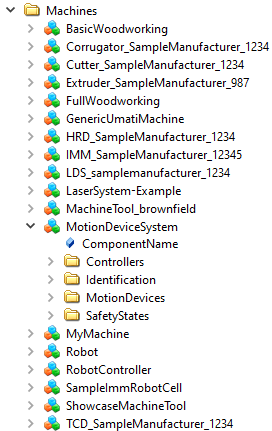
\includegraphics[height=0.7\linewidth]{res/UAExpert.png}
			\caption{Veröffentlichte Objekte im Maschines Ordner des Sample Servers}
			\label{fig:UAExpert}
		\end{figure}
		
		\subsection{Dashboard OPC UA Client}\label{ch:OPCClient}
		
		% Configuration
		Der OPC UA Client hat die Aufgabe, die Daten des Servers an den MQTT Broker weiterzugeben. Für diese Aufgabe stellt der VDMA das \textit{Dashboard-OPCUA-Client} Repository auf GitHub zur Verfügung. Der OPC UA Client läuft in einem Dockercontainer. Er verbindet sich zunächst mit dem OPC UA Server und identifiziert alle Maschinen, die er finden kann. Daraufhin konvertiert er die Daten in eine Json-Datei und schickt sie an den MQTT Broker weiter.
		
		% Spezifikationen
		Der OPC UA Client muss über eine configuration.json so angepasst werden, dass er den richtigen OPC UA Server und MQTT Broker findet. Außerdem wird in dieser Datei ebenfalls festgelegt, nach welchen Spezifikationen während der Identifikation geschaut werden soll. In diesem Fall muss nur nach Maschinen gesucht werden, welche die OPC for Robotics Spezifikation implementieren. In Anhang 1 ist die volle Konfigurationsdatei für einen OPC UA Client für die Robotics Spezifikation.
		
		Um den Client mit dem OPC UA Server zu verbinden, muss die Adresse zum Server und die Anmeldedaten, sowie die Anmeldeform eingetragen werden. In diesem Fall liegt OPC UA Server an der Adresse \textit{192.168.0.133} am Port \textit{4840} und veröffentlicht einen Entrypoint unter \textit{/UA}. Der OPC UA Server verwendet die Anmeldeform 1, was keiner Sicherheitsvorkehrung entspricht. Demnach werden keine Anmeldedaten benötigt. Diese Sicherheitseinstellung ist der Standard für den Sample Server von Umati, sollte in einem Produktionsserver jedoch angehoben werden. Aus diesen Informationen ergibt sich für das Feld \textit{OpcUa} der Konfigurationsdatei folgende Werte:
		
		% OPC UA
		\lstinputlisting[firstline=37,lastline=42,frame=single]{res/code/config.json}
		
		Um mit dem MQTT Broker zu kommunizieren, muss ein \textit{Mqtt} Feld angelegt werden. In diesem sollten zunächst die Verbindungsdaten zu einem eignen Test MQTT Broker eingetragen werden, um zu überprüfen, ob der OPC UA Client reibungslos funktioniert. Ist dies der Fall, können die Daten für den Umati MQTT Broker eingetragen werden. Im folgenden Codebeispiel sind alle Parameter eingetragen, die für die Verbindung mit dem Umati MQTT Broker benötigt werden. Der Nutzername und das Password werden auf Nachfrage vom VDMA bereitgestellt.
		
		% MQTT
		\lstinputlisting[firstline=43,lastline=51,frame=single]{res/code/config.json}
		
		\subsection{Umati MQTT Broker und Web-Dashboard}
		
		% Web Dashboard beschreiben -> Wo daten -> Wo meine Maschinen
		Die Daten werden in einem vom VDMA entworfenen Json Format vom Client geschrieben und anschließend vom Broker veröffentlicht. 
		
		%Aufbau Web Dashboard???
	
		\subsection{Security}
		
		% Risiken
		Die Verbindung zum MQTT Broker von Umati ist nicht sicher. Zur Übermittlung wird http verwendet, welches nicht sicher ist. Auch intern ist die Sicherheit nicht hoch genug. Der OPC UA Server verlangt keine Authentifizierung. Allerdings laufen über diese Systeme nur Testdaten, die keine hohe Sicherheit bedürfen. Sollten jedoch Produktionsdaten und Daten, die kritisch für die Maschinenfunktion sind, über die Verbindungen laufen, sollte die Authentifizierung angepasst werden. 
		
		Der OPC UA Server kann eine seiner Authentifizierungsmöglichkeiten implementieren. Neben dem freien Zugang, kann auch mit Nutzername und Passwort oder Zertifikaten gearbeitet werden, um die Sicherheit herzustellen. 
	
	\section{Implementierung eines Internen Prototyps}\label{ch:Implementierung-Intern}
	
		\subsection{Struktur}
		
		% Verwendete Komponenten
		Der zweite Prototyp baut auf dem ersten auf und nutzt dessen OPC UA Server. Die Daten werden von einem OPC UA Client gelesen, welcher sie weiter an einen lokalen MQTT Broker sendet. Der OPC UA Client ist aus demselben Image wie der Client aus dem ersten Prototyp, allerdings sendet er die Daten nicht an einen MQTT Broker im Internet, sondern an einen lokalen. Veröffentlicht der MQTT Broker die Daten, greifen zwei verschieden Clients auf die Daten zu. Telegraf und NodeRed lesen die Daten aus dem Json-Format und schreiben sie in eine Datenbank. Um die Daten zu visualisieren liest Grafana die Datenbank aus, und stellt alles grafisch dar. In Abbildung \ref{fig:Prototyp2} ist der Fluss der Daten und die beteiligten Komponenten dargestellt. Alle Komponenten laufen in einem Dockercontainer.
		
		\begin{figure}[H]
			\centering
			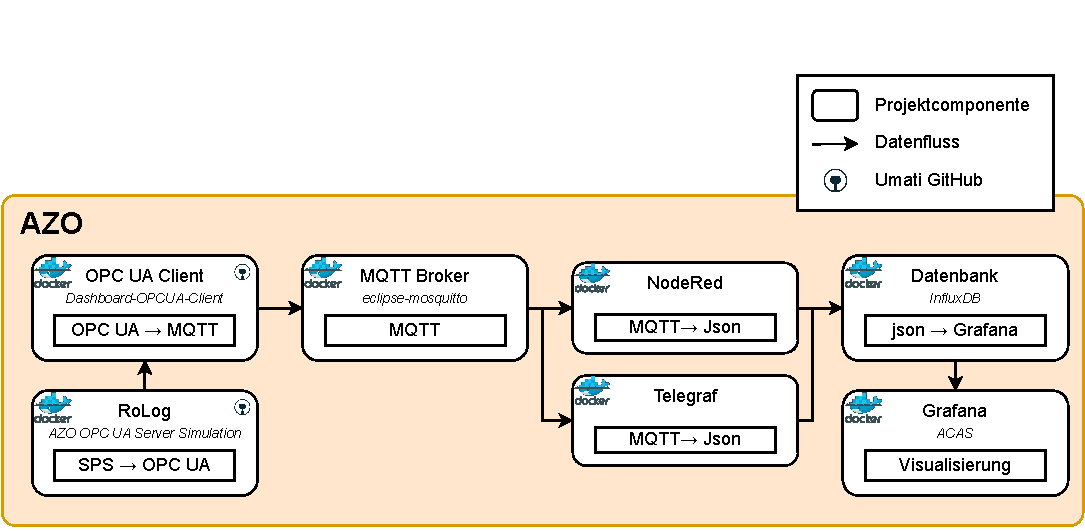
\includegraphics[width=0.9\textwidth]{res/implementierung/Prototyp-Prototyp.pdf}
			\caption{Struktur des zweiten Prototypen}
			\label{fig:Prototyp2}
		\end{figure}
		
		% Portainer
		Neben dem Prototyp läuft ebenfalls eine Portainer Instanz. Diese ist nötig, um auf die InfluxDB Datenbank zuzugreifen, zu können. 
		
		\subsection{OPC UA Server/Client}
		
		% Server
		Um die Daten zu einer internen Visualisierung zu senden, wurde dieselbe Datenquelle verwendet. Der OPC UA Server ist derselbe wie schon in Kapitel \ref{ch:RoLogOPCUA} beschrieben. 
		
		% Client
		Der Client wird aus demselben Repository erstellt, wie auch schon in Kapitel \ref{ch:OPCClient} beschrieben. Allerdings muss nun die \textit{Mqtt}-Konfiguration angepasst werden. Statt der Daten des Umati MQTT Brokers müssen die Verbindungsdaten auf einem lokalen MQTT Server eingetragen werden. In diesem Projekt wurde folgende Konfiguration verwendet:
		
		\lstinputlisting[firstline=52,lastline=60,frame=single]{res/code/config.json}
		
		Der MQTT Broker läuft auf derselben VM mit der Adresse \textit{192.168.0.133} auf dem Port \textit{1883}. Die Daten werden unter dem \textit{umati/v2} Topic veröffentlicht. 
		
		\subsection{MQTT Broker}\label{ch:MQTT Broker}
		
		% MQTT Broker Image
		Wie alle anderen Komponenten des Prototyps ist der MQTT Broker ebenfalls in einen Dockercontainer eingefasst. Er wurde aus dem offiziellen eclipse-mosquitto Image auf Docker Hub erstellt. Der Broker selbst verlangt keine Konfiguration, da die Clients die Daten auf dem Broker veröffentlichen und lesen. Deshalb kann der Default-Container verwendet werden und muss nur an einem Port veröffentlicht werden.
		
		% Befehl zum Starten
		Um den Broker zu starten, kann folgender Befehl auf dem Hostsystem ausgeführt werden:
		
		\begin{lstlisting}[numbers=none, language=bash, frame=single]
			docker run -it -p 1883:1883 -p 9001:9001 eclipse-mosquitto
		\end{lstlisting}
	
		% Befehlerklärung
		Der Befehl nutzt zwei Ports, über die eine Verbindung zum Broker aufgebaut werden kann. Über den Port 1883 kann ein Client über das MQTT Protokoll zugreifen. Der Port 9001 ermöglicht die Verbindung über Websockets. Das \textit{-it} Flag steht für --interactive und verhindert, dass der Container beendet wird, wenn er keine Befehle zum Ausführen mehr hat. Tauscht man dieses Flag mit \textit{-itd} aus, wird der Container als interactive und detatched gestartet.
		
		% Überprüfung
		
		\subsection{InfluxDB}
		
		% Hinführung
		Um die Daten der Sensoren abzuspeichern wird eine influxDB verwendet. Dies ist ein Datenbank Managment System, das sich auf die Abspeicherung und Effiziente Verarbeitung von Zeitreihen spezialisierte. Auch dieses Projekt besitzt ein offizielles Image auf DockerHub (influxdb) welches für den Prototyp verwendet wird. Die Datenbank wird über ein Docker-Compose Datei gestartet. Der Eintrag des Service ist im folgenden Codeausschnitt der \textit{influx.yaml} abgebildet.
		
		\lstinputlisting[firstline=15,lastline=26,frame=single]{res/code/influx.yaml}
		
		% Erklärung Docker Compose File
		Das Docker Compose File erstellt einen Container aus dem influxdb Image der Version 1.8 mit dem Namen \textit{influxdb}. Der restart Parameter ist auf always gestellt, um sicherzustellen, dass der influxdb Container auch nach einem Absturz erneut startet. In den Umgebungsvariablen werden Datenbankname und ein Admin-User angegeben. Die Datenbank läuft auf dem Port \textit{8086} und wird auf den selben Port des Hostsystems geschalten. Der letzte Befehl definiert ein Volume. 
		
		% Volumes
		Volumes sind Speicher, die ein Verzeichnis oder eine Datei innerhalb eines Containers mit einem Verzeichnis des Hostsystems Synchronisieren. Dies ermöglicht die persistente Speicherung von Daten. InfluxDB speichert ebenfalls Daten ab, weshalb ein neues Volume festgelegt werden muss. Am ende der Docker Compose wird ein Volume angelegt, auf das aus dem influxDB Service verwiesen wird. Im folgenden Codesegment werden zwei Volumes erstellt. Eines für die InfluxDB und eines für Grafana, da der Grafanacontainer in der selben Docker Compose Datei erstellt wird.
		
		\lstinputlisting[firstline=44,lastline=46,frame=single]{res/code/influx.yaml}
		
		Um die Daten der Sensoren abzuspeichern, wird eine InfluxDB verwendet. Dies ist ein Datenbankmanagementsystem, das sich auf die Abspeicherung und effiziente Verarbeitung von Zeitreihen spezialisierte. Auch dieses Projekt besitzt ein offizielles Image auf DockerHub (influxdb) welches für den Prototyp verwendet wird. Die Datenbank wird über ein Docker-Compose Datei gestartet. Der Eintrag des Service ist im folgenden Codeausschnitt der \textit{influx.yaml} abgebildet.
		
		\lstinputlisting[firstline=15,lastline=26,frame=single]{res/code/influx.yaml}
		
		% Erklärung Docker Compose File
		Das Docker-Compose File erstellt einen Container aus dem influxdb Image der Version 1.8 mit dem Namen \textit{influxdb}. Der Restart Parameter ist auf always gesetzt, um sicherzustellen, dass der Influxdb-Container auch nach einem Absturz erneut startet. In den Umgebungsvariablen werden Datenbankname und ein Admin-User angegeben. Die Datenbank läuft auf dem Port \textit{8086} und wird auf denselben Port des Hostsystems geschaltet. Der letzte Befehl definiert ein Volume. 
		
		% Volumes
		Volumes sind Speicher, die ein Verzeichnis oder eine Datei innerhalb eines Containers mit einem Verzeichnis des Hostsystems synchronisieren. Dies ermöglicht die persistente Speicherung von Daten. InfluxDB speichert ebenfalls Daten ab, weshalb ein neues Volume festgelegt werden muss. Am Ende der Docker-Compose wird ein Volume angelegt, auf das aus dem InfluxDB-Service verwiesen wird. Im folgenden Codesegment werden zwei Volumes erstellt. Eines für die InfluxDB und eines für Grafana, da der Grafanacontainer in derselben Docker-Compose Datei erstellt wird.
		
		\lstinputlisting[firstline=44,lastline=46,frame=single]{res/code/influx.yaml}
		
		Um die Daten aus dem MQTT Broker zu lesen und in die InfluxDB zu schreiben, können zwei Methoden verwendet werden. NodeRed ist eine Low-Code-Plattform, mit der grafisch Datenflüsse programmiert werden können. Es verwendet Codeblocks, um Anweisungen zu speichern. Telegraf ist ein Open-Source-Server-Agent und Datenverarbeitungsframework, das von der Firma InfluxData entwickelt wurde. Es wurde speziell für die Erfassung, Verarbeitung und Übertragung von Metriken und Ereignisdaten entwickelt und ist ein wichtiger Bestandteil des InfluxData-Ökosystems. 
		
			\subsubsection{NodeRed}
			
			NodeRed läuft ebenfalls in einem Docker-Container. Das offizielle Image von NodeRed ist auf DockerHub abgespeichert. Um den Container, in dem die Entwicklungsumgebung für NodeRed läuft, zu starten, wurde erneut eine Docker-Compose Datei erstellt. 
			
			\lstinputlisting[firstline=3,lastline=11,frame=single]{res/code/NodeRed.yaml}
			
			Es wird ein Node-Red Container aus dem neusten Image erstellt, welches als Umgebungsvariable die Zeitzone benötigt. Um auf den Container zugreifen zu können, wird der Port 1880 des Hostsystems mit dem Container verbunden. Über das Volume werden die Daten des Containers persistent abgespeichert, indem der Ordner \textit{/data} aus dem Container auf einen Speicherort des Hostsystems synchronisiert wird. Dieser Ordner kann frei gewählt werden.
			
			Um einen NodeRed Flow zu erstellen, muss über den Browser auf die Adresse des Containers navigiert werden. Diese stellt sich aus der Adresse des Hostsystems und dem durchgegebenen Port des Containers zusammen (192.168.0.133:1880). Es öffnet sich ein Fenster, in dem ein Flow angelegt werden kann.
			
			Um mit einer InfluxDB kommunizieren zu können, benötigt man das \textit{node-red-contrib-influxdb} Paket. Dieses kann über das Menü (oben rechts) in den Einstellungen installiert werden. Dafür muss auf den Reiter \textit{Palette} Navigiert werden, und der Paketname gesucht und das Paket installiert werden. Nach erfolgreicher Installation sollten neben den MQTT-Nodes auch die InfluxDB-Nodes, wie in Abbildung \ref{fig:nodes} dargestellt, vorhanden sein.
			
			\begin{figure}[H]
				\centering
				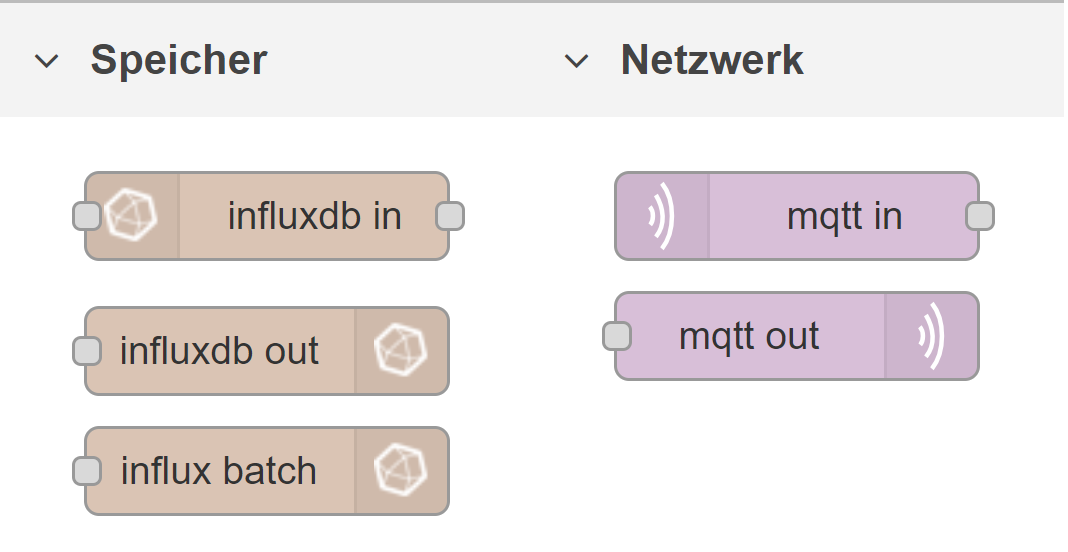
\includegraphics[width=0.6\textwidth]{res/NodeRedNodes.png}
				\caption{Node-Red-Nodes des node-red-contrib-influxdb Packages zur Kommunikation mit influxDB (links) und die Standard MQTT Nodes (rechts)}
				\label{fig:nodes}
			\end{figure}
		
			Der Flow, der die Daten in die InfluxDB schreibt, besteht aus drei Nodes welche in Abbildung \ref{fig:flow} abgebildet sind. Die \textit{mqtt in} Node liest die Daten aus dem MQTT Broker und gibt sie an eine \textit{change} Node weiter. Diese liest die Json-Datei, die sie bekommt, aus und entnimmt alle Parameter, welche relevant für die Darstellung sind. Die letzte Node ist eine \textit{influxdb out}. Sie sendet die Parameter an die InfluxDB und beendet den Flow damit. 
			
			\begin{figure}[H]
				\centering
				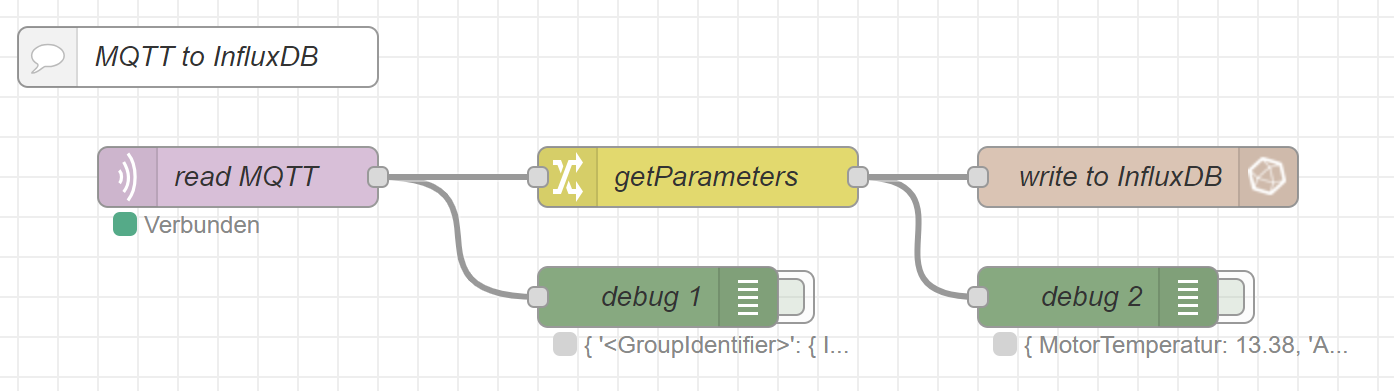
\includegraphics[width=0.9\textwidth]{res/NodeRedFlow.png}
				\caption{NodeRedFlow zur Datenübertragung von MQTT Broker in InfluxDB}
				\label{fig:flow}
			\end{figure}
			
			Mit einem Doppelklick öffnet sich das Eigenschaftsfenster der Node. Die Verbindung zum MQTT Broker wird innerhalb der ersten Node anhand der Server Eigenschaft konfiguriert. Die folgende Liste beinhaltet alle Parameter, welche angepasst werden müssen, um sich mit dem zuvor aufgesetzten MQTT Broker (Kapitel \ref{ch:MQTT Broker}) zu verbinden.
			
			\begin{itemize}
				\item \textbf{Server} $\rightarrow$ Bearbeiten:
				\subitem \textbf{Server}: 192.168.0.133
				\subitem \textbf{Port}: 1883
				\item \textbf{Topic}: umati/v2/rolog/ControllerType/nsu=http:\_2F\_2Fvdma.org\_2FOPCRobotics\linebreak TestServer\_2F;i=5002
				\item \textbf{Ausgang}: Ein analysiertes (parsed) JSON-Objekt
			\end{itemize}
			Der Name des Servers und der Node können frei gewählt werden.
			
			Die zweite Node liest die richtigen Daten aus den MQTT Daten aus und passt sie für eine eigene Json-Datei an. Dafür müssen zunächst alle Daten aus der \textit{payload} ausgelesen, und in eigene Variablen übersetzt werden. In Abbildung \ref{fig:NodeRedChange} ist auf der rechten Seite das Auslesen und Abspeichern der Motortemperatur abgebildet. Es können auch ganze Objekte in Zwischenvariablen abgespeichert werden. Pfad zur Motortemperatur:
			
			\textit{payload["<MotionDeviceIdentifier>"].Robot.PowerTrains["<PowerTrainIdentifier>"]\linebreak.PowerTrain1["<MotorIdentifier>"].Motor1.ParameterSet.MotorTemperature}
			
			\begin{figure}[H]
				\centering
				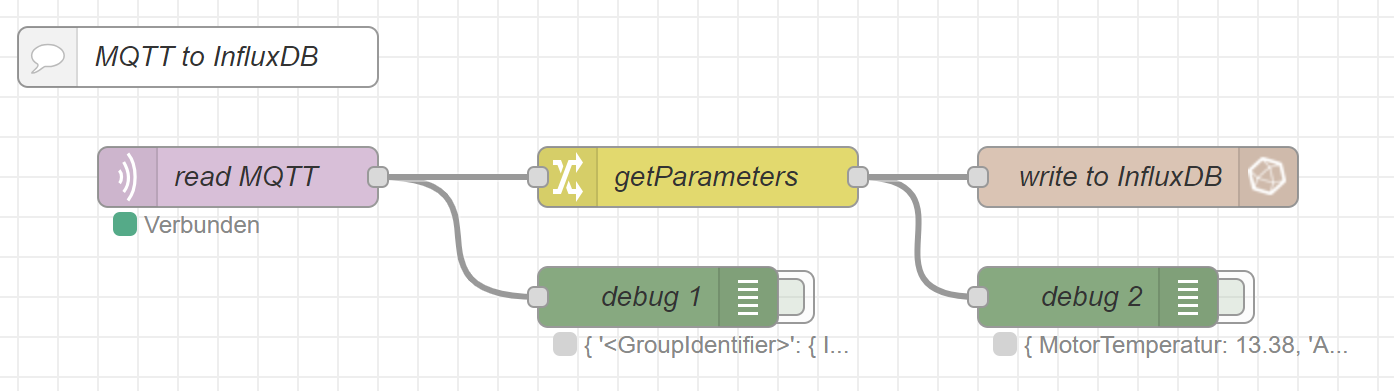
\includegraphics[width=0.9\textwidth]{res/NodeRedFlow.png}
				\caption{Auslesen einer Zwischenvariable (links) und zusammenführen dieser (rechts) in einer Change Node.}
				\label{fig:NodeRedChange}
			\end{figure}
			
			Das Zusammenführen der Informationen erfolgt durch die Verwendung des JSONata Felds. Hierbei kann ein neues Json-Objekt in die Payload geschrieben und die zuvor erstellten Zwischenvariablen verwendet werden. Es kann auch auf die Zwischenvariablen verzichtet und direkt auf die Json-Datei des MQTT Brokers zugegriffen werden, allerdings vermindert dies die Übersichtlichkeit. Das folgende Codebeispiel beinhaltet den Wert, der in die rechte Regel aus Abbildung \ref{fig:NodeRedChange} eingefügt werden muss.
			
			\begin{lstlisting}[numbers=none, frame=single]
				{
					"MotorTemperatur": MotorTemp.value,
					"Axis1-Acc": Axis1.ActualAcceleration.value,
					"Axis2-Acc": Axis2.ActualAcceleration.value,
					"Axis1-Pos": Axis1.ActualPosition.value,
					"Axis2-Pos": Axis2.ActualPosition.value,
					"Axis1-Speed": Axis1.ActualSpeed.value,
					"Axis2-Speed": Axis2.ActualSpeed.value
				}
			\end{lstlisting}
		
			Anhand der Debug-Nodes kann die Payload zwischen jeder Node ausgelesen werden. Dadurch kann sichergestellt werden, dass das Übertragen der Werte durch die \textit{Change}-Node funktioniert hat. 
			
			Die letzte Node sendet nun die Json-Datei an die InfluxDB. Folgende Konfigurationen müssen im Eigenschaftenfenster der \textit{influxdb out} angepasst werden:
			
			\begin{itemize}
				\item \textbf{Server} $\rightarrow$ Bearbeiten:
				\subitem \textbf{Version}: 1.8-flux
				\subitem \textbf{URL}: http://192.168.0.133:8086
				\item \textbf{Database}: influx
				\item \textbf{Measurement}: NodeRed
			\end{itemize}
			
			Sobald die Daten an die InfluxDB gesendet werden, wird eine Database mit der Bezeichnung \textit{influx} und eine Measurment namens \textit{NodeRed} erstellt. Die Daten liegen darin ab und können anschließend von Grafana ausgelesen werden.
			
			\subsubsection{Telegraf}
		
				Sobald die Daten an die InfluxDB gesendet werden, wird eine Database mit der Bezeichnung \textit{influx} und eine Measurment namens \textit{NodeRed} erstellt. Die Daten liegen darin ab und können anschließend von Grafana ausgelesen werden.
			
			\subsubsection{Telegraf}
			
			Anstatt von NodeRed kann auch Telegraf verwendet werden, um Daten aus einem MQTT Broker zu lesen und in eine InfluxDB zu speichern. Um einen Dockercontainer mit Telegraf zu erstellen, wurde folgende Konfiguration in einer Docker-Compose gespeichert.
			
			\lstinputlisting[firstline=3,lastline=14,frame=single]{res/code/influx.yaml}
			
			Diese Konfiguration erstellt einen Container mit der Bezeichnung telegraf aus dem neusten telegraf Image. Für die Kommunikation mit dem Container wird der Port \textit{8125} verwendet. Da Telegraf auf eine laufende InfluxDB voraussetzt, wird der Parameter \textit{depends\_on} auf den Namen des InfluxDB-Containers gesetzt. Beide Anwendungen werden zeitgleich gestartet, da sie in derselben Docker-Compose Datei definiert werden, jedoch wartet Telegraf darauf, dass InfluxDB läuft, bevor er startet. Sollte während der Laufzeit ein Fehler passieren oder die InfluxDB neu gestartet werden, so versucht der Telegraf Container aufgrund des \textit{restart} Parameters immer neu zu starten. Das \textit{links} Keyword verbindet die beiden Container miteinander. Docker öffnet dadurch für die Kommunikation einen sicheren Tunnel.
			
			Telegraf muss noch zusätzlich zu den Docker-Compose Informationen eine Konfigurationsdatei mitgegeben werden. Dafür wird ein Volume verwendet, der die Konfigurationsdatei beim Starten in den Container abspeichert. Diese Konfigurationsdatei beinhaltet Datenquelle, den MQTT Broker, und Datenziel, die InfluxDB. Zusätzlich können hier auch Veränderungen an den Daten vorgenommen werden. Beispielsweise kann nur ein bestimmtes Objekt an die InfluxDB weitergegeben werden. 
			
			Anhang II beinhaltet die gesamte Konfigurationsdatei. Zunächst müssen allgemeine Umgebungsvariablen für Telegraf gesetzt werden. Dem Agenten muss der eigene Hostname mitgeteilt werden. 
			
			\lstinputlisting[firstline=12,lastline=12,frame=single]{res/code/telegraf.conf}
			
			Im Folgenden Code ist die Datenquelle konfiguriert. Zunächst muss die Adresse und die Verbindungsintervalle angegeben werden. Außerdem werden alle Topics angegeben, die Telegraf abonnieren soll. In diesem Fall stehen hier die Topics der drei Maschinenkomponenten, die der Umati Server simuliert. Der letzte Parameter beschreibt das Datenformat, in welchem die Daten auf dem MQTT Broker abliegen
			
			\lstinputlisting[firstline=22,lastline=34,frame=single]{res/code/telegraf.conf}
			
			Um die Daten an die Datenbank zu versenden, muss Adresse, Datenbank und Anmeldekriterien angegeben werden. Der Telegraf Container meldet sich mit den gegebenen Anmeldedaten an und erstellt eine Database \textit{influx} und ein Measurment namens \textit{measurments}. Dort liegen dann alle Daten, die der MQTT Broker veröffentlicht. 
			
			\lstinputlisting[firstline=15,lastline=20,frame=single]{res/code/telegraf.conf}
			
			Nachdem die Konfigurationsdatei vollständig ist, kann der Container gestartet werden. Stürzt er direkt wieder ab, muss die Verbindung überprüft werden, da Telegraf entweder die InfluxDB oder den MQTT Broker nicht finden kann.
		
		\subsection{Grafana}
		
		% Docker
		Der Grafana Container wird gemeinsam mit dem Telegraf und InfluxDB Containern gestartet. Der folgende Codeausschnitt ist aus der Docker-Compose entnommen. Es wird ein Container der neusten Version von Grafana erstellt. Zum Zeitpunkt des Projektes ist Version 8.2.6 die aktuellste. Aus dem Image von DockerHub wird ein Container erstellt, der den Namen grafana-server bekommt. Er wird aufgrund des \textit{depends\_on} nach der influxDB gestartet und öffnet einen sicheren Kommunikationskanal zur Datenbank über \textit{links}. In den Umgebungsvariablen müssen Authentifizierungsdaten für einen Admin angegeben werden und es können Plugins angegeben werden, die installiert werden sollen. Der Container bekommt ein Volume zugeteilt und wird am Port \textit{3000} des Hostsystems veröffentlicht. 
		
		\lstinputlisting[firstline=27,lastline=42,frame=single]{res/code/influx.yaml}
		
		Ist der Container erfolgreich gestartet, kann über den Browser auf den Port 3000 navigiert werden und die grafische Oberfläche von Grafana öffnet sich. Zunächst muss InfluxDB als Datenquelle eingebunden, im Anschluss ein Dashboard erstellt, und die Anfragen an die Datenbank eingefügt werden. 
		
		\subsection{Datenquelle}
		
		% Datenquelle
		Um den zuvor erstellten InfluxDB Container als Quelle einzubinden, muss in den Einstellungen auf \textit{Data sources} navigiert werden. Unter \textit{Add new connection} kann InfluxDB als Abfragesprache, die URL des Containers und die Admin Anmeldedaten eingetragen werden. Außerdem muss die gewünschte Database angegeben werden. Da sich InfluxDB und Grafana im selben Dockernetzwerk befinden, kann als URL \textit{http://influxdb:8086} eingetragen werden. Die Adresse zum Container ist der Containername, wodurch die Kommunikation nur Docker intern stattfindet. Die Database ist \textit{influx}, da der Telegraf Agent und NodeRed die Daten in diese Database speichern.
		
		
		\subsection{Erstellen eines Diagramms}
		
		Für ein Diagramm muss ein Dashboard erstellt werden. Dies kann unter dem Menüpunkt \textit{Dashboards} $\rightarrow$ \textit{New} erstellt werden. Auf dem Dashboard kann über die \textit{Add} Schaltfläche ein neues Dashboard erstellt werden.
		
		In Abbildung \ref{fig:GrafanaDiagramm} ist das Bearbeitungsfenster für ein Diagramm abgebildet. Es besteht aus drei Komponenten. Einem Test-Diagramm (oben-links), welches die eingegebenen Parameter live übernimmt und darstellt, wie das Diagramm auf dem Dashboard aussehen wird. Eine Design-Toolbar (rechts), welches das Aussehen und die angezeigten Daten des Diagramms visuell verändert. Die Anfragen an die Datenbank werden über das Datenfenster (unten-links) abgesetzt. Es können zwei Arten von Abfragen erstellt werden. Entweder direkte Testabfragen, in denen der Nutzer eine vollständige Abfrage als String absetzen muss und einen Baukasten. Der Baukasten ist deutlich einfacher zu nutzen und vor allem bei einfachen Abfragen sehr hilfreich. Werden die Abfragen jedoch zu komplex, kann es hilfreich sein, einen eigenen Befehl zu formulieren.
		
		In Abbildung \ref{fig:GrafanaDiagramm} ist die Abfrage an die InfluxDB abgebildet, die die Beschleunigung einer Roboterachse ausliest. Diese Daten wurden über NodeRed in die Datenbank eingelesen und anhand des Grafana-Baukastens portiert. 
		
		\begin{figure}[H]
			\centering
			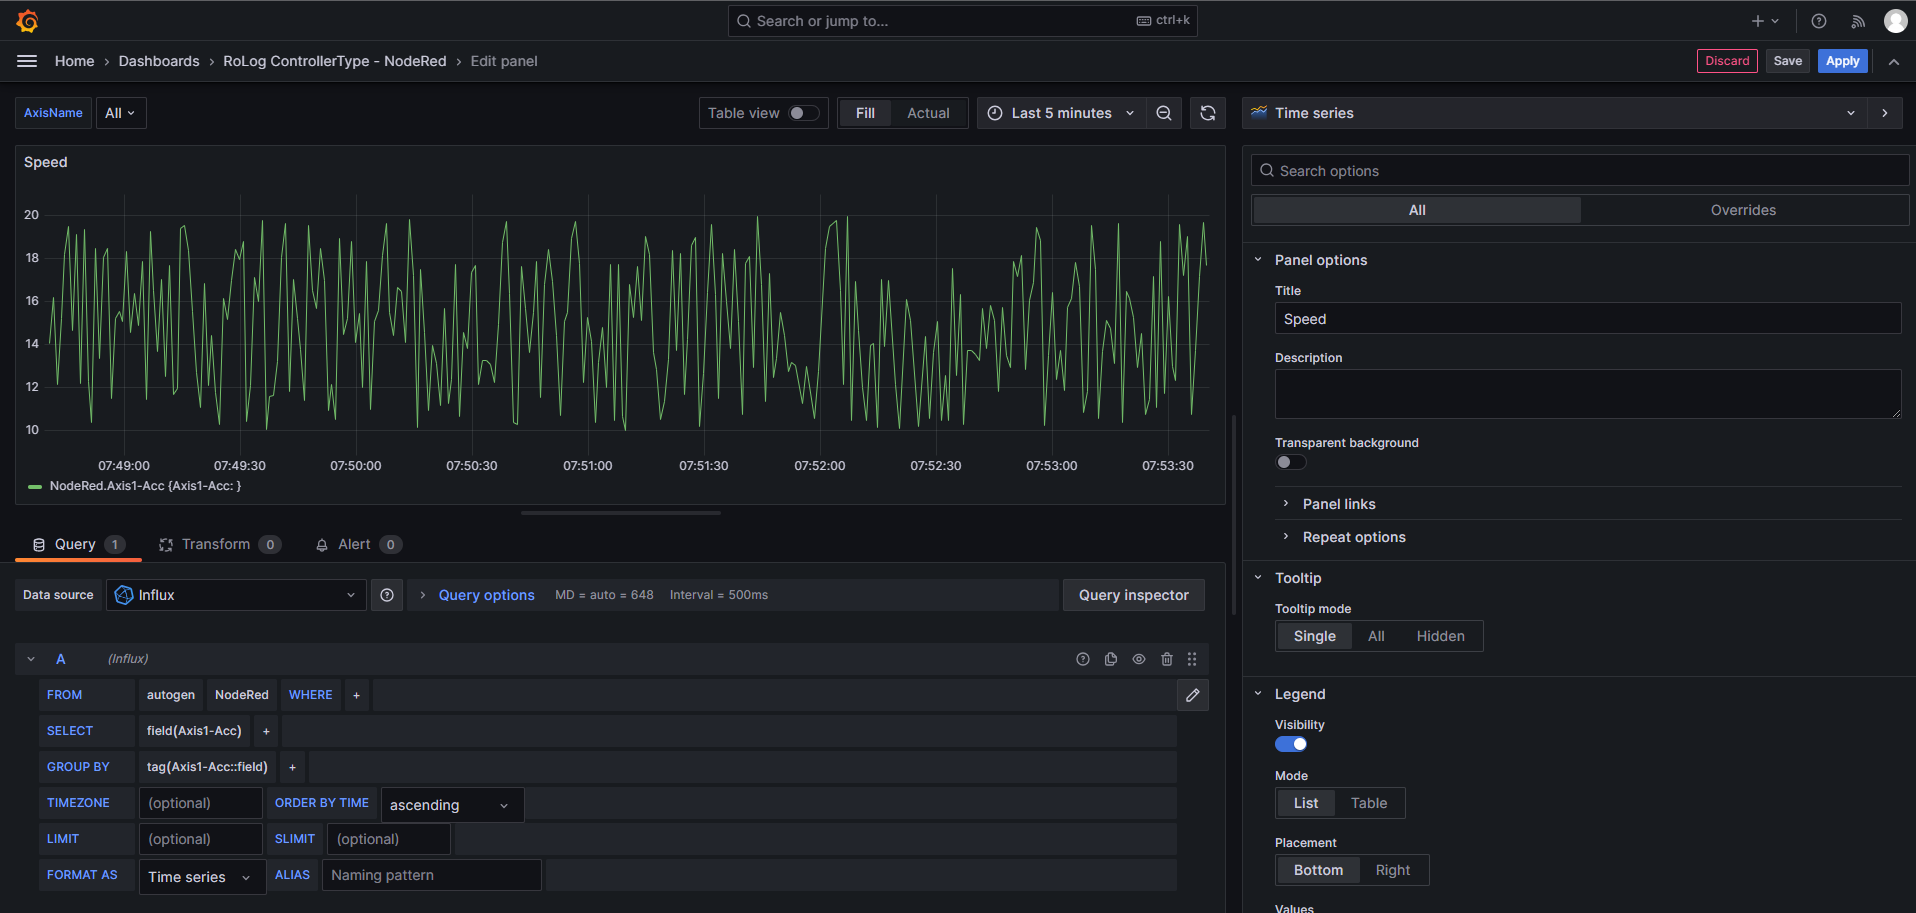
\includegraphics[width=0.9\textwidth]{res/Grafana-Diagramm.png}
			\caption{Bearbeitungsfenster eines Grafana Dashboards.}
			\label{fig:GrafanaDiagramm}
		\end{figure}
	
		An dem Design des Diagramms wurden keine Veränderungen vorgenommen. Alle Dashboards verwenden die Defaulteinstellungen für Diagramme. Sollten Anpassungen notwendig oder erwünscht sein, können sie im rechten Menü vorgenommen werden.
		
			\subsubsection{NodeRed}\label{ch:NodeRedGrafana}
			
			Um Daten aus der InfluxDB zu lesen, muss die richtige Datenquelle und Database angegeben werden. Da die Daten bereits in NodeRed transformiert wurden, erfolgt die Abfrage in Grafana sehr einfach. In Abbildung \ref{fig:noderedabfrage} ist die Abfrage über den Baukasten abgebildet. Als \textit{Data source} wird die zuvor angelegte Datenquelle von influx verwendet. Die Tabelle in denen die Daten liegen ist NodeRed und das gewünschte Feld kann über ein Dropdown-Menü ausgewählt werden. 
		
		\begin{figure}[H]
			\centering
			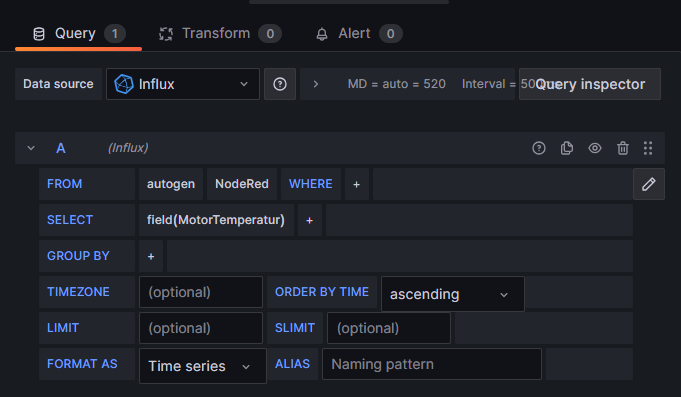
\includegraphics[width=0.9\linewidth]{res/NodeRedAbfrage.png}
			\caption{Abfrage der Motortemperatur der von NodeRed gelieferten Daten}
			\label{fig:noderedabfrage}
		\end{figure}
		
		Über das Stiftsymbol auf der rechten Seite des Editors öffnet sich ein Klartextfeld, in dem der Befehl weiter angepasst werden kann. Alle anderen Werte, die über NodeRed in die Datenbank gespeichert wurden, können wie die Motortemperatur angezeigt werden.
		
		Das Einlesen der Daten über NodeRed hat den Vorteil, dass die Abfrage in Grafana sehr einfach und leicht lesbar ist. Allerdings benötigt die Konfiguration in NodeRed und das Transformieren der Daten viel manuelle Arbeit. NodeRed ist eine gute Entscheidung, wenn bereits Kenntnisse in NodeRed vorhanden sind und die InfluxDB möglichst wenige Daten abspeichern soll. 
		
		\subsubsection{Telegraf}
		
		% Abfrage
		Telegraf überträgt alle Daten der Json, die vom MQTT Broker veröffentlicht werden, in die Datenbank. Die Zeitreihe hat dadurch enorm viele Felder, die Grafana im Anschluss ausfiltern muss. In Abbildung \ref{fig:telegrafabfrage} ist die Abfrage für die Motortemperatur abgebildet. In diesem Fall wird der Texteditor zum Erstellen der Abfrage genutzt, allerdings kann auch der Baukasten verwendet werden, wie in Kapitel \ref{ch:NodeRedGrafana} beschrieben, genutzt werden. Telegraf benennt die Felder nach dem Pfad in der Json und damit entsteht sehr lange Namen. Wie in Kapitel \ref{ch:NodeRedGrafana} muss die Datenquelle \textit{Influx} angegeben werden. Es muss die Database \textit{mqtt\_consumer} und das erwünschte Feld verwendet werden.
		
		\begin{figure}[H]
			\centering
			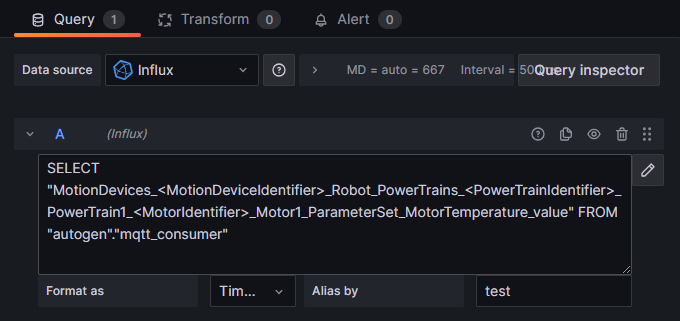
\includegraphics[width=0.9\linewidth]{res/TelegrafAbfrage.png}
			\caption{Abfrage der Motortemperatur der von Telegraf gelieferten Daten}
			\label{fig:telegrafabfrage}
		\end{figure}
		
		Telegraf hat den Vorteil, dass alle Werte aus der Json, die der MQTT Broker veröffentlicht, in Grafana ausgewählt werden können. Zwar kann die Json in der Telegraf Konfigurationsdatei angepasst werden, allerdings ist die mit einem hohen Programmieraufwand verbunden, wenn die Json so komplex ist wie in diesem Beispiel. Der Nachteil von Telegraf ist es, da durch die nicht transformierten Daten, die in die InfluxDB gespeichert werden, auch viele Felder bei Grafana ankommen. Die Abfrage für die Daten im Diagramm werden dadurch schnell unübersichtlich und lange, können jedoch mehr Datenpunkte einfacher integrieren.
		
		NodeRed und Telegraf sind beides sinnvolle Ansätze zur Übertragung von Daten in die InfluxDB und Grafana. Ihre Vor- und Nachteile sollten abgewogen werden und je nach Bedürfnis angewandt werden. Bei NodeRed fällt die Auswahl der Felder in den NodeRed-Flow während bei der Methode mit Telegraf die Auswahl erst in Grafana vorgenommen wird.
		
		\subsection{Dashboardanpassungen}
		
		Um die Dashboards dynamischer zu gestalten, kommen Variablen und Rows zum Einsatz. Dies ist ein Feature von Grafana, welches die dynamische Veränderung von Datenbankanfragen und Designs ermöglicht. Für das finale Dashboard wurde eine Variable angelegt, welche alle möglichen Achsen des Roboters beinhaltet. Variablen in Grafana funktionieren wie Arrays, welche ein oder mehrere Werte beinhalten. Alle Diagramme mit Anfragen für eine Achse werden in einer Row zusammengefasst, welche die zuvor erstellte Variable als \textit{Repeat for} nutzt. Dies bewirkt, dass für jede Achse, welche unter der Variable ausgewählt wurde, eine eigene Row erstellt. Durch das Anpassen der Abfragen kann erreicht werden, dass für jede Achse ein eigenes Diagramm erstellt wird.
		
		In Abbildung \ref{fig:variables} ist eine Abfrage an die von NodeRed gelieferten Daten. Durch das Verwenden der Variable \textit{\${AxisName}} wird die Anfrage in jeder Row für jeden Wert der Variable einzeln durchgeführt.
		
		\begin{figure}[H]
			\centering
			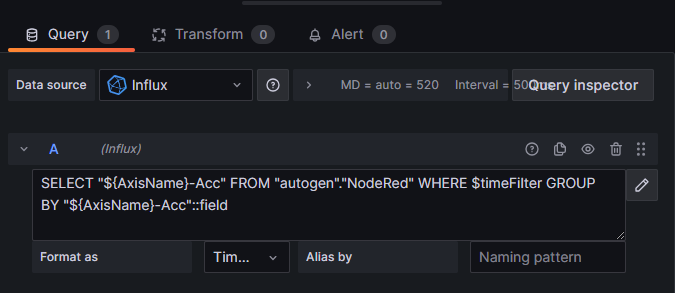
\includegraphics[width=0.9\linewidth]{res/variables.png}
			\caption{Datenbankabfrage mit Verwendung von Variable}
			\label{fig:variables}
		\end{figure}
			
	\chapter{Fazit und Diskussion}\label{ch:Diskussion_Fazit}
	
		% (2-5 Seiten)	
	
		% Disskussion -> Subjektive Bewertung der Spezifikation UMATI, ... Literaturpunkte meine Meinung, Sinnvoll Einzusetzen
	
	\printbibliography
	\frontmatter
	
	\pagebreak
	\chapter{Anhänge} %TODO: Alle Codebeispiele rein, Yaml Files ...
	\section*{Anhang I: configuration.json}
	\lstinputlisting{res/code/config.json}
	\pagebreak
	\section*{Anhang II: telegraf.conf}
	\lstinputlisting{res/code/telegraf.conf}
	\pagebreak

\end{document}
